% =====================================================================
%  CodeTwin AI -- research paper (IEEE conference format)
%  Group P6, Dept. of CSE (Data Science), TSSM's PVPIT, Pune
%
%  main.tex is generated from main.template.tex by pilot/paper_numbers.py:
%  every number about our study comes from pilot/results/results.json.
%  Edit the template, not main.tex, if you change text around numbers.
% =====================================================================

\documentclass[conference]{IEEEtran}
\IEEEoverridecommandlockouts

\usepackage{cite}
\usepackage{amsmath,amssymb,amsfonts}
\usepackage{algorithm}
\usepackage{algpseudocode}
\usepackage{graphicx}
\usepackage{textcomp}
\usepackage{xcolor}
\usepackage{booktabs}
\usepackage{array}
\usepackage{url}
\usepackage{balance}
\usepackage{tikz}
\usetikzlibrary{positioning,arrows.meta,fit}


\makeatletter
\newcommand{\linebreakand}{%
  \end{@IEEEauthorhalign}
  \hfill\mbox{}\par
  \mbox{}\hfill\begin{@IEEEauthorhalign}
}
\makeatother


\begin{document}

\title{CodeTwin AI: Evidence-Aware, Risk-Calibrated\\
Regression Test Selection with Abstention---\\
A Survey and an Empirical Study on Python Projects}

\author{
\IEEEauthorblockN{Aarya Godbole}
\IEEEauthorblockA{\textit{Dept. of CSE (Data Science)} \\
\textit{TSSM's PVPIT}\\
Pune, India \\
aaryagodbole550@gmail.com}
\and
\IEEEauthorblockN{Suhani Bhati}
\IEEEauthorblockA{\textit{Dept. of CSE (Data Science)} \\
\textit{TSSM's PVPIT}\\
Pune, India \\
bhatisuhani5@gmail.com}
\and
\IEEEauthorblockN{Madhura Suryawanshi}
\IEEEauthorblockA{\textit{Dept. of CSE (Data Science)} \\
\textit{TSSM's PVPIT}\\
Pune, India \\
suryawanshimadhura51@gmail.com}
\linebreakand
\IEEEauthorblockN{Shreya Gole}
\IEEEauthorblockA{\textit{Dept. of CSE (Data Science)} \\
\textit{TSSM's PVPIT}\\
Pune, India \\
shreyakgole@gmail.com}
\and
\IEEEauthorblockN{Dr. T. A. Kamble}
\IEEEauthorblockA{\textit{Dept. of CSE (Data Science)} \\
\textit{TSSM's PVPIT}\\
Pune, India \\
tulsiram17@gmail.com}
}

\maketitle

% =====================================================================

% =====================================================================
\begin{abstract}
Running the entire test suite after each change is slow, and AI coding assistants increase the number of changes. Regression test selection (RTS) runs only the tests a change may affect, but current techniques return a fixed set without stating how much risk remains, and they assume that dependencies they cannot resolve do not exist. After reviewing 27 related works, we propose CodeTwin AI, which ranks tests with a learned risk model, estimates the remaining risk of each selection, calibrates its threshold to a target miss rate using conformal risk control, and abstains to a broader selection when the estimated risk is too high. We evaluated a Python prototype on 681 changes across 8 open-source projects using three ground truths: per-test coverage, 812 detected seeded faults and the ground truth published by NameRTS. Calibration based on older commits failed under drift: at a 10\% target, 17.5\% of later changes missed tests that should have run. With adaptive conformal inference, observed miss rates were 4.5\%, 9.3\% and 19.9\% for targets of 5\%, 10\% and 20\%. Abstaining when the risk estimate exceeded the target caught 26 of the 31 changes on which line-coverage selection was unsafe, whereas rule-based triggers caught only 7, and gave 98.2\% safe changes while saving 29.7\% of test time. The learned ranking did not outperform a coverage ranking, and file-level coverage alone was safe on these projects. A selection's residual risk can be stated and held at a chosen level, but only with calibration that adapts over time.
\end{abstract}


\begin{IEEEkeywords}
abstention, adaptive conformal inference, change impact analysis, conformal risk control, mutation testing, regression test selection
\end{IEEEkeywords}


% =====================================================================
\section{Introduction}\label{sec:intro}
% =====================================================================

% P1 -- Context and motivation
Whenever a developer makes changes to the code, regression testing ensures that things that previously worked still work~\cite{yoo2012survey}. However, this can become expensive on large projects: the whole test suite must be run after each change, causing delays and putting pressure on continuous integration (CI)~\cite{elbaum2014ci,memon2017taming}. By skipping tests we can save time, but we may miss exactly the test that the change breaks. AI coding assistants make this worse by creating patches faster than they can be verified. One preprint ran an agent on the SWE-bench Verified benchmark using a locally hosted open-weight model and saw it create regressions; telling the agent which tests might be affected reduced them~\cite{alonso2026tdad}. This is early evidence, not a general result about AI-written code, but it shows how important it is to know which tests are relevant. Regression test selection (RTS) runs only part of the test suite, so we must also know how likely the selection is to miss an affected test.

% P2 -- Existing approaches, limitations, and research gaps
RTS selects tests to run based on the dependencies between the changed code and the tests. A selection is \emph{safe} when it keeps every test the change could affect~\cite{legunsen2016static}. Ekstazi (Gligoric et al.) tracks which files each test accesses and re-runs a test only if one of those files has changed~\cite{gligoric2015ekstazi}. Liu et al.\ reasoned about semantics-modifying changes so that tests affected only by certain such changes need not be re-run~\cite{liu2023finerts}. JcgEks uses dynamic file dependencies plus static method call graphs~\cite{zhang2024jcgeks}. These methods all target Java. Python is harder, because importing modules can execute code and dynamic features make it unclear which function a call will reach. NameRTS uses name matching and run-time probing to handle this issue, and it included every affected test file on 99.6\% of 500 commits across ten projects~\cite{wang2026namerts}. Predictive test selection (PTS) is a different approach that learns from past results which tests are likely to fail~\cite{machalica2019pts}.

Across the literature we see three gaps. First, although average results are good, they do not tell us how much risk remains in a specific selection, and PTS thresholds based on historical samples should not be read as guarantees for a single commit~\cite{machalica2019pts}. Second, dependency evidence may be incomplete without explaining why: NameRTS documents limitations involving \texttt{eval}, library code, and a test affected through an external-library callback~\cite{wang2026namerts}. Third, weak evidence for the current change does not necessarily widen the selection. NameRTS selects all tests if a registry decorator changes~\cite{wang2026namerts}, and PTS may rely on running the whole suite periodically~\cite{machalica2019pts}. Statistics can offer a solution. Conformal risk control can bound the expected value of monotone losses, such as the miss rate, under assumptions that include exchangeability~\cite{angelopoulos2024crc}. Conformal methods have also been used for abstention on language-model hallucinations~\cite{yadkori2024abstention} and for prioritising tests in CI~\cite{altinisik2026conformal}. As far as we know, none of the reviewed techniques combines risk calibration, visible dependency limitations and a fallback to a broader selection when uncertain.

% P3 -- Research question and methodology
This paper asks: \emph{can evidence-aware test selection with calibrated abstention keep the miss rate at a chosen target while running substantially fewer tests than the full suite, and does it flag the changes on which conventional selection fails?} We study this first on Python projects. To answer it, we design and implement CodeTwin AI, a Python prototype, and compare it with established baselines on the commit histories of open-source projects. Changes are processed in time order, so every decision is based only on earlier information from the same project.

% Objectives (from the project synopsis)
The project has five objectives: (O1)~create an evidence graph that shows how files, functions, tests and other repositories are connected and how each link was discovered; (O2)~select tests by risk within a time budget; (O3)~estimate the risk remaining in a selection, calibrated to a target miss rate, and abstain when there is not enough evidence; (O4)~integrate with the developer workflow and AI coding agents; and (O5)~evaluate against established baselines on public projects. This paper implements the evidence collection of O1 and the selection, calibration and abstention of O2 and O3 for single Python repositories, and evaluates them as O5. The evidence store of O1 and first versions of the O4 interfaces have since been implemented in the CodeTwin AI tool (release 0.1.0) but are not evaluated here. Cross-repository links have been designed but not yet implemented.

% P4 -- Contributions and principal findings
We make four contributions.
\begin{itemize}
    \item A survey of 27 works on test selection, coverage, call graphs, calibrated prediction and testing support for AI agents, highlighting the gap between efficient selection and knowing how much risk remains (Sections~\ref{sec:related} and~\ref{sec:gap}).
    \item CodeTwin AI, which treats unresolved dependencies as uncertainty, ranks tests by learned risk per second, estimates the residual risk $r(c)$ of each selection, and calibrates its threshold with conformal risk control that adapts to drift. If the risk is too high, it abstains to a broader run (Sections~\ref{sec:approach} and~\ref{sec:impl}).
    \item An evaluation on 681 changes across 8 Python projects with three ground truths: per-test coverage, 812 seeded faults and, on 3 projects, the published ground truth and selections of NameRTS. We compare against ten baselines, including the published NameRTS selections (Sections~\ref{sec:setup} and~\ref{sec:results}). Calibration based on older commits failed under drift, while adaptive calibration kept the observed miss rate at or below the target on the history projects and close to it on the shorter NameRTS histories. Risk-based abstention caught most unsafe changes with far fewer false alarms than rule-based triggers.
    \item A replication package archived on Zenodo, containing the scripts, the GitHub Actions workflows, the data collected for every change and every reported number.
\end{itemize}

% P5 -- Paper organisation
Section~\ref{sec:background} introduces key concepts and a motivating example. Section~\ref{sec:related} reviews prior work and Section~\ref{sec:gap} states the research gap. Sections~\ref{sec:approach} and~\ref{sec:impl} present the approach and its implementation, Sections~\ref{sec:setup} and~\ref{sec:results} the evaluation, Section~\ref{sec:discussion} the implications, Section~\ref{sec:threats} the threats to validity and Section~\ref{sec:conclusion} the conclusions.

% =====================================================================
\section{Background and Motivating Example}\label{sec:background}
% =====================================================================
\subsection{Key Concepts}
\textit{Regression test selection} (RTS) runs only a selected subset of the tests when code changes, rather than all of them. A selection is said to be \textit{safe} if it excludes no test that can fail because of the change~\cite{yoo2012survey}. \textit{Test prioritisation} is a process that reorders tests but never excludes any~\cite{yoo2012survey}. To identify the relevant tests, \textit{change impact analysis} is used, that is, the process of finding the affected functions, files, tests and repositories. Change impact analysis can be either \textit{static} (analysing code without executing it) or \textit{dynamic} (monitoring the code as it runs). Static analysis cannot trace calls made through \texttt{getattr} and \texttt{importlib}, whereas dynamic analysis considers only the paths that were executed during the run. \textit{Per-test code coverage} records all lines run by each test; thus, the tests covering a change, and the changed lines not covered by any test, can be found.

An ideal tool would also provide an assessment of how risky its decision is. The \textit{miss rate} is the fraction of changes for which at least one test that should have been run was excluded. A risk estimate is considered \textit{calibrated} if the estimated probability of an event matches its actual frequency; e.g., changes estimated as 5\% risky should be missed approximately 5\% of the time. \textit{Conformal risk control} uses held-out data to find a threshold that keeps the expected miss rate below the selected target~\cite{angelopoulos2024crc}. The guarantee provided by conformal risk control depends on the \textit{exchangeability} of calibration changes and future changes, an assumption that commits ordered in time do not necessarily satisfy. \textit{Adaptive conformal inference} therefore adjusts the target level online after each observed error, so that the long-run error rate follows the target level regardless of data drift~\cite{gibbs2021aci}. \textit{Abstention} means that the system admits uncertainty about its prediction~\cite{yadkori2024abstention}; in our context, the system then suggests running additional tests rather than a small subset. Lastly, \textit{mutation testing} introduces tiny artificial faults, called mutants, into the program, and a test detects (kills) a mutant if it fails on it; mutant detection is a popular and widely validated proxy for fault detection~\cite{jia2011mutation,just2014mutants}.
\subsection{Motivating Example}
Consider the scenario in Fig.~\ref{fig:example}. A pull request renames the field \texttt{price} of \texttt{orders.Order} within a shared library, and all of the library's tests pass. The change has four dependants, each known in a different way: \texttt{billing.total()} is a static caller in the same repository; \texttt{vendor\_portal/pricing.py} is a consumer in another repository, declared in an OpenAPI contract; \texttt{customer\_app/cart.py} is a consumer in another repository that is seen only at run time and has no tests; and \texttt{plugins.load()} uses \texttt{getattr}, so its target cannot be determined statically. The line style in the figure shows how each connection was found. A conventional tool links the change to two tests, \texttt{test\_billing.py} and \texttt{test\_pricing.py}, and reports it as ``verified''. However, it misses the untested consumer and the unresolved call. CodeTwin AI instead highlights these two blind spots, reports the remaining risk, which they push above a 5\% target, and suggests running more tests. Passing tests in the changed repository therefore do not mean the change is safe. The following sections explain how CodeTwin AI gathers this evidence and turns it into such a suggestion.

\begin{figure}[t]
\centerline{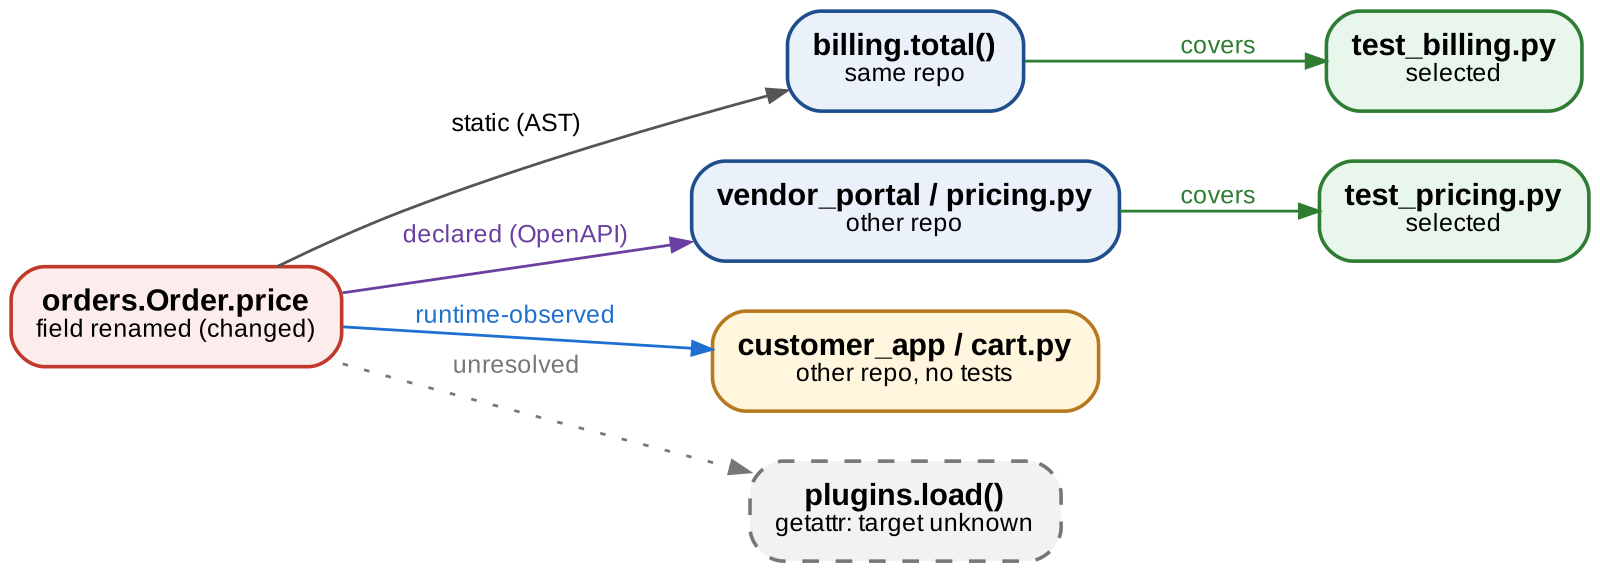
\includegraphics[width=\columnwidth]{figures/example.png}}
\caption{Impact map for renaming \texttt{orders.Order.price} (red). Line style shows how each link was found: static analysis (AST), a declared OpenAPI contract, runtime observation, or unresolved (dotted). Green nodes are the selected tests, the orange node is a consumer with no tests, and the dashed node, \texttt{plugins.load()}, uses \texttt{getattr}, so its target is unknown.}
\label{fig:example}
\end{figure}

% =====================================================================
\section{Related Work}\label{sec:related}
% =====================================================================
We searched Google Scholar, arXiv, the ACM Digital Library and IEEE Xplore for work on regression test selection, change impact analysis, static and dynamic dependency analysis, test coverage, learning-based test selection, conformal prediction, abstention and testing support for AI coding agents. We were interested in papers published at ISSTA, ASE, ICSE, FSE and ICLR. We focused on work from 2015--2026 but also included some earlier foundational studies. We kept 27 works that are foundational or closest to our problem, and we did not aim for exhaustive coverage. We organise them into six themes: foundations, precise and hybrid selection, coverage and change structure, Python selection, learning-based selection and test generation, and calibration, abstention and AI coding agents. Table~\ref{tab:survey} summarises the reviewed works.


\subsection{Foundations of Regression Test Selection}
Yoo and Harman~\cite{yoo2012survey} distinguish between test-suite minimisation, regression test selection (RTS) and test-case prioritisation; RTS re-runs only the tests that a change may affect. Rothermel and Harrold~\cite{rothermel1996analyzing} proposed a framework for comparing selection techniques, whose criteria are inclusiveness (a fully inclusive technique is safe), precision, efficiency and generality. Ekstazi tracks which files each test uses at run time and re-runs a test if one of those files has changed. On 615 revisions of 32 projects it reduced end-to-end testing time by 32\% on average compared with running all tests~\cite{gligoric2015ekstazi}. Legunsen et al.\ studied static selection on 985 revisions of 22 projects. They found that a class-level technique performed comparably to Ekstazi but was sometimes unsafe, while a method-level technique performed poorly~\cite{legunsen2016static}. STARTS is a Maven tool for static class-level selection that needs no instrumentation or runtime information. The authors report that it selected on average 35.2\% of tests, with an end-to-end time of 81.0\% of running all tests~\cite{legunsen2017starts}. Unlike Ekstazi, the static technique does not need a test run to collect dependencies. These studies report safety and time savings as aggregates over revisions, not as a calibrated estimate of the risk left by the selection for a single change. The kind of dependency evidence therefore decides both how much time is saved and when tests can be skipped safely.

\subsection{Precise and Hybrid Selection}
Using file-level dependencies keeps analysis cheap, but tests may be selected that the change cannot affect. Ekstazi, for example, selected more tests than FaultTracer (a method-level tool) on the six projects where both ran, yet had a much lower end-to-end time~\cite{gligoric2015ekstazi}. Liu et al.\ analysed changes in five projects. They found that some semantics-modifying changes need not trigger tests that only they affect, and built FineEkstazi and FineSTARTS on this finding. On 1,150 versions of 23 projects, the variants selected on average 41.7\% and 31.8\% fewer test classes and took 33.7\% and 28.7\% less end-to-end time than Ekstazi and STARTS, respectively, with no new safety violations reported by RTSCheck~\cite{liu2023finerts}. JcgEks combines Ekstazi's dynamic file dependencies with static method call graphs and is designed to handle callbacks from external libraries safely. On 1,000 revisions of 20 projects, it selected 29.0\% fewer test classes and took 30.9\% less end-to-end time than Ekstazi, without missing any test class in the authors' safety check. Compared with FineEkstazi, it had a similar end-to-end time and number of selected test classes, while FineEkstazi was confirmed to miss test classes~\cite{zhang2024jcgeks}. HyRTS combines method-level and file-level analysis; on 2,707 revisions of 32 projects it outperformed file-level selection in selected test ratio and offline testing time~\cite{zhang2018hyrts}. These techniques depend on their dependency model, language support and handling of unresolved dependencies. In the evaluations we checked, safety and savings are reported as aggregates, not as a risk estimate for a single change, and this is the gap that CodeTwin AI addresses.

\subsection{Coverage and Change Structure}
Prioritisation orders tests instead of excluding them. Rothermel et al.\ ordered tests by total coverage, additional coverage or estimated fault-revealing ability, and compared the rate of fault detection with untreated, random and optimal orders~\cite{rothermel2001prioritizing}. However, coverage can be expensive to refresh after every change. iJaCoCo, built on Ekstazi and JaCoCo, runs a minimal subset of tests to update only the coverage affected by a change. On 1,122 versions of 22 repositories it sped up end-to-end coverage analysis by 1.86$\times$ on average and up to 8.20$\times$ compared with JaCoCo; it was faster on 17 of the 22 repositories and selected 47.34\% of test classes, against 20.63\% for Ekstazi~\cite{wang2024ijacoco}. Altiero et al.\ use tree kernels on abstract syntax trees to quantify structural change and prioritise tests. On five real-world Java projects, using 100 fault-injected variants per version pair (over 5,000 scenarios), they report better prioritisation effectiveness than well-known techniques with typically negligible overhead~\cite{altiero2024treekernel}. Ivankovi\'c et al.\ describe coverage at Google, applied to changesets and code review, with five years of adoption data and 512 survey responses from 3,000 developers~\cite{ivankovic2019coverage}; this is evidence from industrial practice rather than a controlled experiment. Executing a line does not show that a test will detect a fault, and none of these works estimates the risk of a selection. Coverage has a scope and a collection time, and structural change is a complementary signal. CodeTwin AI uses coverage from the previous commit together with structural change features.

\subsection{Selection for Python}
Python makes dependency analysis harder: modules execute code when they are imported, and many call targets are unknown until run time. PyCG generates static call graphs by tracking assignments across modules. On a micro-benchmark of 112 small programs it was complete on 111 and sound on 103, but on five real-world packages it reached about 99.2\% precision and only about 69.9\% recall~\cite{salis2021pycg}. Roughly 30\% of real call edges were therefore missing from the graph, so any selection technique built on it would miss those edges and assume that there is no dependency. NameRTS is a selection technique that does not use call graphs. It uses a bipartite graph of code elements and names, and selects a test when a modified code element can be reached from a name that the test uses~\cite{wang2026namerts}. On a new dataset of 500 commits from ten projects it skipped 69.9\% of test files on average and reduced end-to-end testing time by 45.6\%, and it selected all affected tests on 99.6\% of commits, whereas the file-level baseline was safe on only 76.6\%. NameRTS is conservative by design, but its answer is still binary: it gives no information about how risky a particular commit is, and its misses, although rare, are not shown to the developer. Coverage-based selection has also been used for Python. Kauhanen et al.\ integrated a coverage-based selection tool into their continuous integration pipeline and evaluated it with mutation testing on three open-source projects; the selected subsets missed 0--2\% of faults at file level but 16--24\% at line level~\cite{kauhanen2021python}. For prioritisation, pytest-ranking reorders pytest suites; on 4,308 GitHub Actions builds of 14 Python projects it revealed failures sooner than the default and random orders with little overhead~\cite{cheng2025pytestranking}. In dynamic languages a sizeable share of real dependencies is hidden from static analysis, and a selection technique should reveal this instead of hiding it.

\subsection{Machine-Learning-Based Selection and Test Generation}
Machine-learning-based techniques replace explicit dependencies with learned models. Machalica et al.\ built a model that predicts, from historical test results at Meta, which tests a change is likely to break. Deployed in production, it caught more than 95\% of individual test failures and more than 99.9\% of faulty changes while halving the infrastructure cost of testing~\cite{machalica2019pts}. These are aggregate measures: the selection threshold is set from historical samples, and the developer gets no information about how risky their own change is. Bertolino et al.\ compared ten machine-learning algorithms for regression testing in continuous integration. They contrasted learning-to-rank with ranking-to-learn (reinforcement learning) on subjects from the Apache Commons project, and analysed which properties of the code and of the test process decide which approach works better~\cite{bertolino2020learning}. Language models have also been used to generate tests. Harman et al.\ describe ACH at Meta, which generates mutants for one concern, such as privacy, and then generates tests that detect them. Applied to 10,795 Android Kotlin classes across seven platforms, it generated 9,095 mutants and 571 privacy-hardening tests, and engineers accepted 73\% of the tests offered in test-a-thons~\cite{foster2025ach}. Machine learning therefore helps to prioritise and generate tests, but its confidence is aggregate, and the language-model output was useful only after it had been verified by execution and by engineers.

\subsection{Calibration, Abstention and AI Coding Agents}
Conformal methods provide distribution-free guarantees using a held-out calibration set; Angelopoulos and Bates present them for practitioners~\cite{angelopoulos2023gentle}. Conformal risk control extends conformal prediction to guarantee that the expected value of any monotone loss, such as the false-negative rate, stays at or below a user-chosen level, assuming exchangeability~\cite{angelopoulos2024crc}. Abbasi Yadkori et al.\ used conformal prediction to decide when a language model should abstain. On two question-answering datasets their method kept the hallucination rate within the bound, and on long answers it abstained much less often than log-probability baselines~\cite{yadkori2024abstention}. Shahini et al.\ applied conformal prediction to two just-in-time defect predictors on the Qt and OpenStack datasets. At 95\% confidence the guarantee was met for only 27\% and 9\% of their predictions, although the method filtered out most of their false positives and false negatives~\cite{shahini2024jitcp}. Alt{\i}n{\i}{\c{s}}{\i}k combined history-based prioritisation in continuous integration with adaptive conformal calibration. On 273 failing jobs across four Java projects, calibration reduced the candidate set from about 32\% to about 26\% of the tests while keeping about 91\% of the failing tests~\cite{altinisik2026conformal}. This work prioritises tests, but it does not bound the residual risk of a selection for each change.

AI coding agents make this gap a practical problem. SWE-bench contains 2,294 real issues from 12 Python repositories; when it was introduced, the best model resolved 1.96\% of them~\cite{jimenez2024swebench}. Venkatesh et al.\ evaluated 24 language models and found that static tools such as PyCG still produced more complete and sound call graphs~\cite{venkatesh2025llmcg}; model output therefore cannot replace analysis. TDAD gives an agent a static mapping from code to tests before it commits a patch. On 100 SWE-bench Verified instances with a locally hosted open-weight model (Qwen3-Coder 30B), it reduced the test-level regression rate from 6.08\% to 1.82\%~\cite{alonso2026tdad}. However, the mapping carries no calibrated confidence, and the agent is never told to stop. Calibration and abstention methods with guarantees exist, and agents need support for test selection, but in our search the two have not been combined.

\begin{table*}[t]
\caption{Summary of the Reviewed Literature}
\label{tab:survey}
\centering
\footnotesize
\renewcommand{\arraystretch}{1.15}
\begin{tabular}{@{}>{\raggedright\arraybackslash}p{0.06\textwidth}>{\raggedright\arraybackslash}p{0.22\textwidth}>{\raggedright\arraybackslash}p{0.19\textwidth}>{\raggedright\arraybackslash}p{0.22\textwidth}>{\raggedright\arraybackslash}p{0.21\textwidth}@{}}
\toprule
\textbf{Work} & \textbf{Approach} & \textbf{Evaluation} & \textbf{Key finding} & \textbf{Limitation for our problem} \\
\midrule
\cite{yoo2012survey} & Minimisation, selection and prioritisation survey & Literature review & Distinguishes three testing problems & No risk estimate \\
\cite{rothermel1996analyzing} & Safety and precision criteria & Framework & Foundation for comparing RTS techniques & Not per-change risk \\
\cite{gligoric2015ekstazi} & Dynamic file-based dependency selection & 615 revisions, 32 projects & 32\% less end-to-end time & No residual-risk estimate \\
\cite{legunsen2016static} & Static class- and method-level selection & 985 revisions, 22 projects & Comparable to Ekstazi at class level & Sometimes unsafe at class level \\
\cite{legunsen2017starts} & Static class-based selection tool & Tool demonstration & 35.2\% of tests; 81.0\% of full time & No risk estimate \\
\cite{liu2023finerts} & Semantics-modifying change reasoning & 1,150 versions, 23 projects & 41.7\%/31.8\% fewer test classes & Fixed selection; no risk estimate \\
\cite{zhang2024jcgeks} & Dynamic files plus static call graphs & 1,000 revisions, 20 projects & 29.0\% fewer classes, 30.9\% less time vs.\ Ekstazi & Fixed selection; no risk estimate \\
\cite{zhang2018hyrts} & Hybrid method- and file-level analysis & 2,707 revisions, 32 projects & Outperformed file-level selection & Fixed selection; no risk estimate \\
\cite{rothermel2001prioritizing} & Coverage- and fault-based test ordering & Experiments on program test suites & All orders improved fault-detection rate & Orders tests; does not select \\
\cite{wang2024ijacoco} & Incremental coverage updates & 1,122 versions, 22 repositories & 1.86$\times$ average speedup vs.\ JaCoCo & Coverage is not fault detection \\
\cite{altiero2024treekernel} & AST tree-kernel prioritisation & Five Java projects; 5,000+ scenarios & Better ordering, minimal overhead & Orders tests; does not remove any \\
\cite{ivankovic2019coverage} & Industrial changeset-level coverage & Five years of data; 512 survey responses & Used in code review & Practice study; no proof of fault detection \\
\cite{salis2021pycg} & Static Python call graphs & Micro- and macro-benchmarks & ${\sim}$99.2\% precision, ${\sim}$69.9\% recall (macro) & Edges silently missing \\
\cite{wang2026namerts} & Name-based Python selection & 500 commits, 10 projects & 69.9\% files skipped; safe on 99.6\% & Binary; misses not reported \\
\cite{kauhanen2021python} & Coverage-based Python selection in CI & Mutation testing, 3 projects & Missed 0--2\% of faults (file), 16--24\% (line) & Fixed granularity; no risk estimate \\
\cite{cheng2025pytestranking} & Test prioritisation plugin for pytest & 4,308 CI builds, 14 projects & Finds failures sooner than default order & Orders tests; does not remove any \\
\cite{machalica2019pts} & History-based learned selection & Meta production data & Caught $>$95\% of failures at half the cost & Aggregate confidence only \\
\cite{bertolino2020learning} & Ten ML ranking algorithms in CI & Apache Commons subjects & Context decides the best strategy & Orders tests; no risk estimate \\
\cite{foster2025ach} & LLM mutation-guided test generation & 10,795 Android Kotlin classes & 73\% of tests accepted & Not aimed at selection risk \\
\cite{angelopoulos2023gentle} & Conformal prediction tutorial & Methods and examples & Distribution-free guarantees & Not applied to testing \\
\cite{angelopoulos2024crc} & Conformal risk control & Vision and NLP tasks & Bounds expected monotone loss & Not applied to test selection \\
\cite{yadkori2024abstention} & Conformal abstention for LLMs & Two QA datasets & Bounded hallucination rate & Not applied to code \\
\cite{shahini2024jitcp} & Conformal just-in-time defect prediction & Qt and OpenStack datasets & Guarantee met for 27\%/9\% of predictions & Predicts defects; does not select tests \\
\cite{altinisik2026conformal} & Conformal prioritisation in CI & 273 jobs, 4 Java projects & ${\sim}$91\% failing tests at ${\sim}$26\% of tests & Orders tests; no per-change risk \\
\cite{jimenez2024swebench} & Benchmark of real GitHub issues & 2,294 issues, 12 repositories & Best model resolved 1.96\% & Measures fixes, not regressions \\
\cite{venkatesh2025llmcg} & LLMs for types and call graphs & 24 LLMs, new benchmarks & PyCG outperformed LLMs on call graphs & LLM edges need verification \\
\cite{alonso2026tdad} & Code-to-test mapping for agents & 100 SWE-bench Verified instances, one model & Test-level regressions 6.08\% $\to$ 1.82\% & Uncalibrated; agent never stops \\
\bottomrule
\end{tabular}
\end{table*}


\subsection{Summary and Research Gap}\label{sec:gap}
Table~\ref{tab:gap} compares the closest work with CodeTwin AI by language, multi-repository support, a risk estimate for an individual change, calibrated abstention and blind-spot reporting. There are four observations from this review.
\begin{enumerate}
\item Techniques report safety as an average over many commits: NameRTS, for example, is safe on 99.6\% of commits~\cite{wang2026namerts}, but no information is given about how risky an individual change is.
\item Calls that static analysis cannot resolve, such as those made through \texttt{getattr}, are silently dropped instead of being reported to the developer~\cite{salis2021pycg}.
\item Calibration and abstention with statistical guarantees exist~\cite{angelopoulos2024crc,yadkori2024abstention}, and conformal calibration has been combined with history-based prioritisation in continuous integration~\cite{altinisik2026conformal}, but no technique we found selects tests for a single change with an explicit risk and the option to abstain.
\item Most techniques support one language and one repository: the semantics-aware and hybrid selectors target only Java~\cite{liu2023finerts,zhang2024jcgeks}, NameRTS targets Python~\cite{wang2026namerts}, and none of the techniques reviewed follows dependants into other repositories.
\end{enumerate}
We could not find any technique that combines a residual-risk estimate for an individual change, calibration against a desired miss rate, abstention and explicit blind-spot reporting. Our search was not exhaustive, so we do not claim that no such work exists.
\begin{table}[t]
\caption{Comparison of the Closest Work With CodeTwin AI}
\label{tab:gap}
\centering
\footnotesize
\setlength{\tabcolsep}{1.8pt}
\begin{tabular}{@{}lccccc@{}}
\toprule
\textbf{Work} & \textbf{Lang.} & \textbf{Multi-repo} & \textbf{Risk} & \textbf{Abstain} & \textbf{Blind spots} \\
\midrule
NameRTS & Python & No & No & No & No \\
Predictive Test Sel. & Any & No & Aggregate & No & No \\
Conformal CI ranking & Java & No & No & No & No \\
TDAD & Python & No & Score & No & No \\
\textbf{CodeTwin AI} & Python & Design & Yes & Yes & Yes \\
\bottomrule
\end{tabular}
\end{table}

% =====================================================================
\section{Proposed Approach: CodeTwin AI}\label{sec:approach}
% =====================================================================

\subsection{Problem Formulation}
Let $c$ be a commit that changes some source files of a project whose test suite is $T$. CodeTwin AI selects tests at the file level. The run time $t(i)$ of a test file $i\in T$ is measured on the previous commit; if the test file did not exist before, the median run time is used. Let $A(c)\subseteq T$ be the set of test files that are truly affected by $c$ (defined in Section~\ref{sec:setup}), and let $F(c)\subseteq T$ be the set of test files that $c$ adds or modifies; these are always run. For each commit, the system returns a subset $S(c)$ that satisfies $F(c)\subseteq S(c)$ and a decision, \textsc{Proceed} or \textsc{Abstain}, where abstaining means that a larger set of tests is run (the full suite or a larger evidence-based selection). A commit is \emph{missed} if $A(c)\nsubseteq S(c)$.

There are two modes for this framework. In \emph{budget mode} the developer fixes a time budget $B$, and the selection must satisfy
\begin{equation}
\textstyle\sum_{i\in S(c)} t(i) \le B . \label{eq:budget}
\end{equation}
In \emph{calibrated mode} the developer fixes a target miss rate $\alpha$, and the expected miss rate over future commits must stay at or below that target:
\begin{equation}
\mathbb{E}\big[\,\mathbf{1}\{A(c)\nsubseteq S(c)\}\,\big] \le \alpha . \label{eq:risk}
\end{equation}
We define the probability that a selection misses an affected test as its \emph{residual risk}, and write $r(c)$ for its estimate for one change (Section~\ref{sec:risk}). Calibrated mode bounds the miss rate over many changes; abstention is applied to individual changes whose risk estimate is too high.

Three assumptions have been made. First, tests are selected at the file level: pytest reports run times per file, and most Python projects organise their tests in files. Selecting individual test functions would use the same evidence, but the start-up cost of the test runner would dominate. Second, tests are assumed to be deterministic; flaky tests~\cite{parry2022flaky} are not modelled. Third, the decision for $c$ uses only information that is available before the tests of $c$ run: the diff and static facts of $c$, and the dynamic evidence (coverage and run times) collected on the previous commit. Budgets are usually stated relative to the full suite, so we write $B=b\cdot\sum_{i\in T}t(i)$ with $b\in(0,1]$ and report results for $b\in\{0.10,0.25,0.50\}$.

\subsection{Architecture}
Fig.~\ref{fig:arch} shows the four layers of CodeTwin AI. \emph{Layer~1} collects evidence about a change: the changed lines from the git diff, imports and dynamic-call markers from the language adapters (the Python \texttt{ast} module first, tree-sitter parsers for further languages), per-test coverage and run times from the test runner, declared dependencies from package manifests and API contracts, and, optionally, suggestions from a locally run language model. \emph{Layer~2} stores every finding as an evidence record in a typed dependency graph. \emph{Layer~3} calculates a score for each test file, selects tests within a budget or above a threshold calibrated on recent commits, and abstains if the estimated residual risk is above the desired level (rule-based uncertainty triggers were evaluated as an alternative). \emph{Layer~4} delivers the decision to developers in a VS Code extension and as a pull-request check, and to AI coding agents through a Model Context Protocol (MCP) server. The prototype evaluated in this paper implements the Python parts of Layers~1 and~3 (Section~\ref{sec:impl}); the evidence store, the language-model suggestions and the Layer~4 interfaces are designed but not evaluated here.

This architecture rests on four design decisions. First, the analysis is \emph{local first}: it runs on the developer's machine or the CI runner, and no code is sent outside that machine unless the optional language model is enabled. Second, \emph{transparent models}, logistic regression or gradient boosting, are preferred over deep learning so that every score can be traced back to its features. Third, adding support for a new language should only require an \emph{adapter}, i.e.\ a parser, a test runner and a coverage collector that write evidence in a common format. Everything above Layer~1 is shared, so the framework is independent of the language; currently, only Python is implemented. Lastly, SQLite and NetworkX are used instead of a graph database, which is sufficient for the repository sizes we target.

\begin{figure*}[t]
\centerline{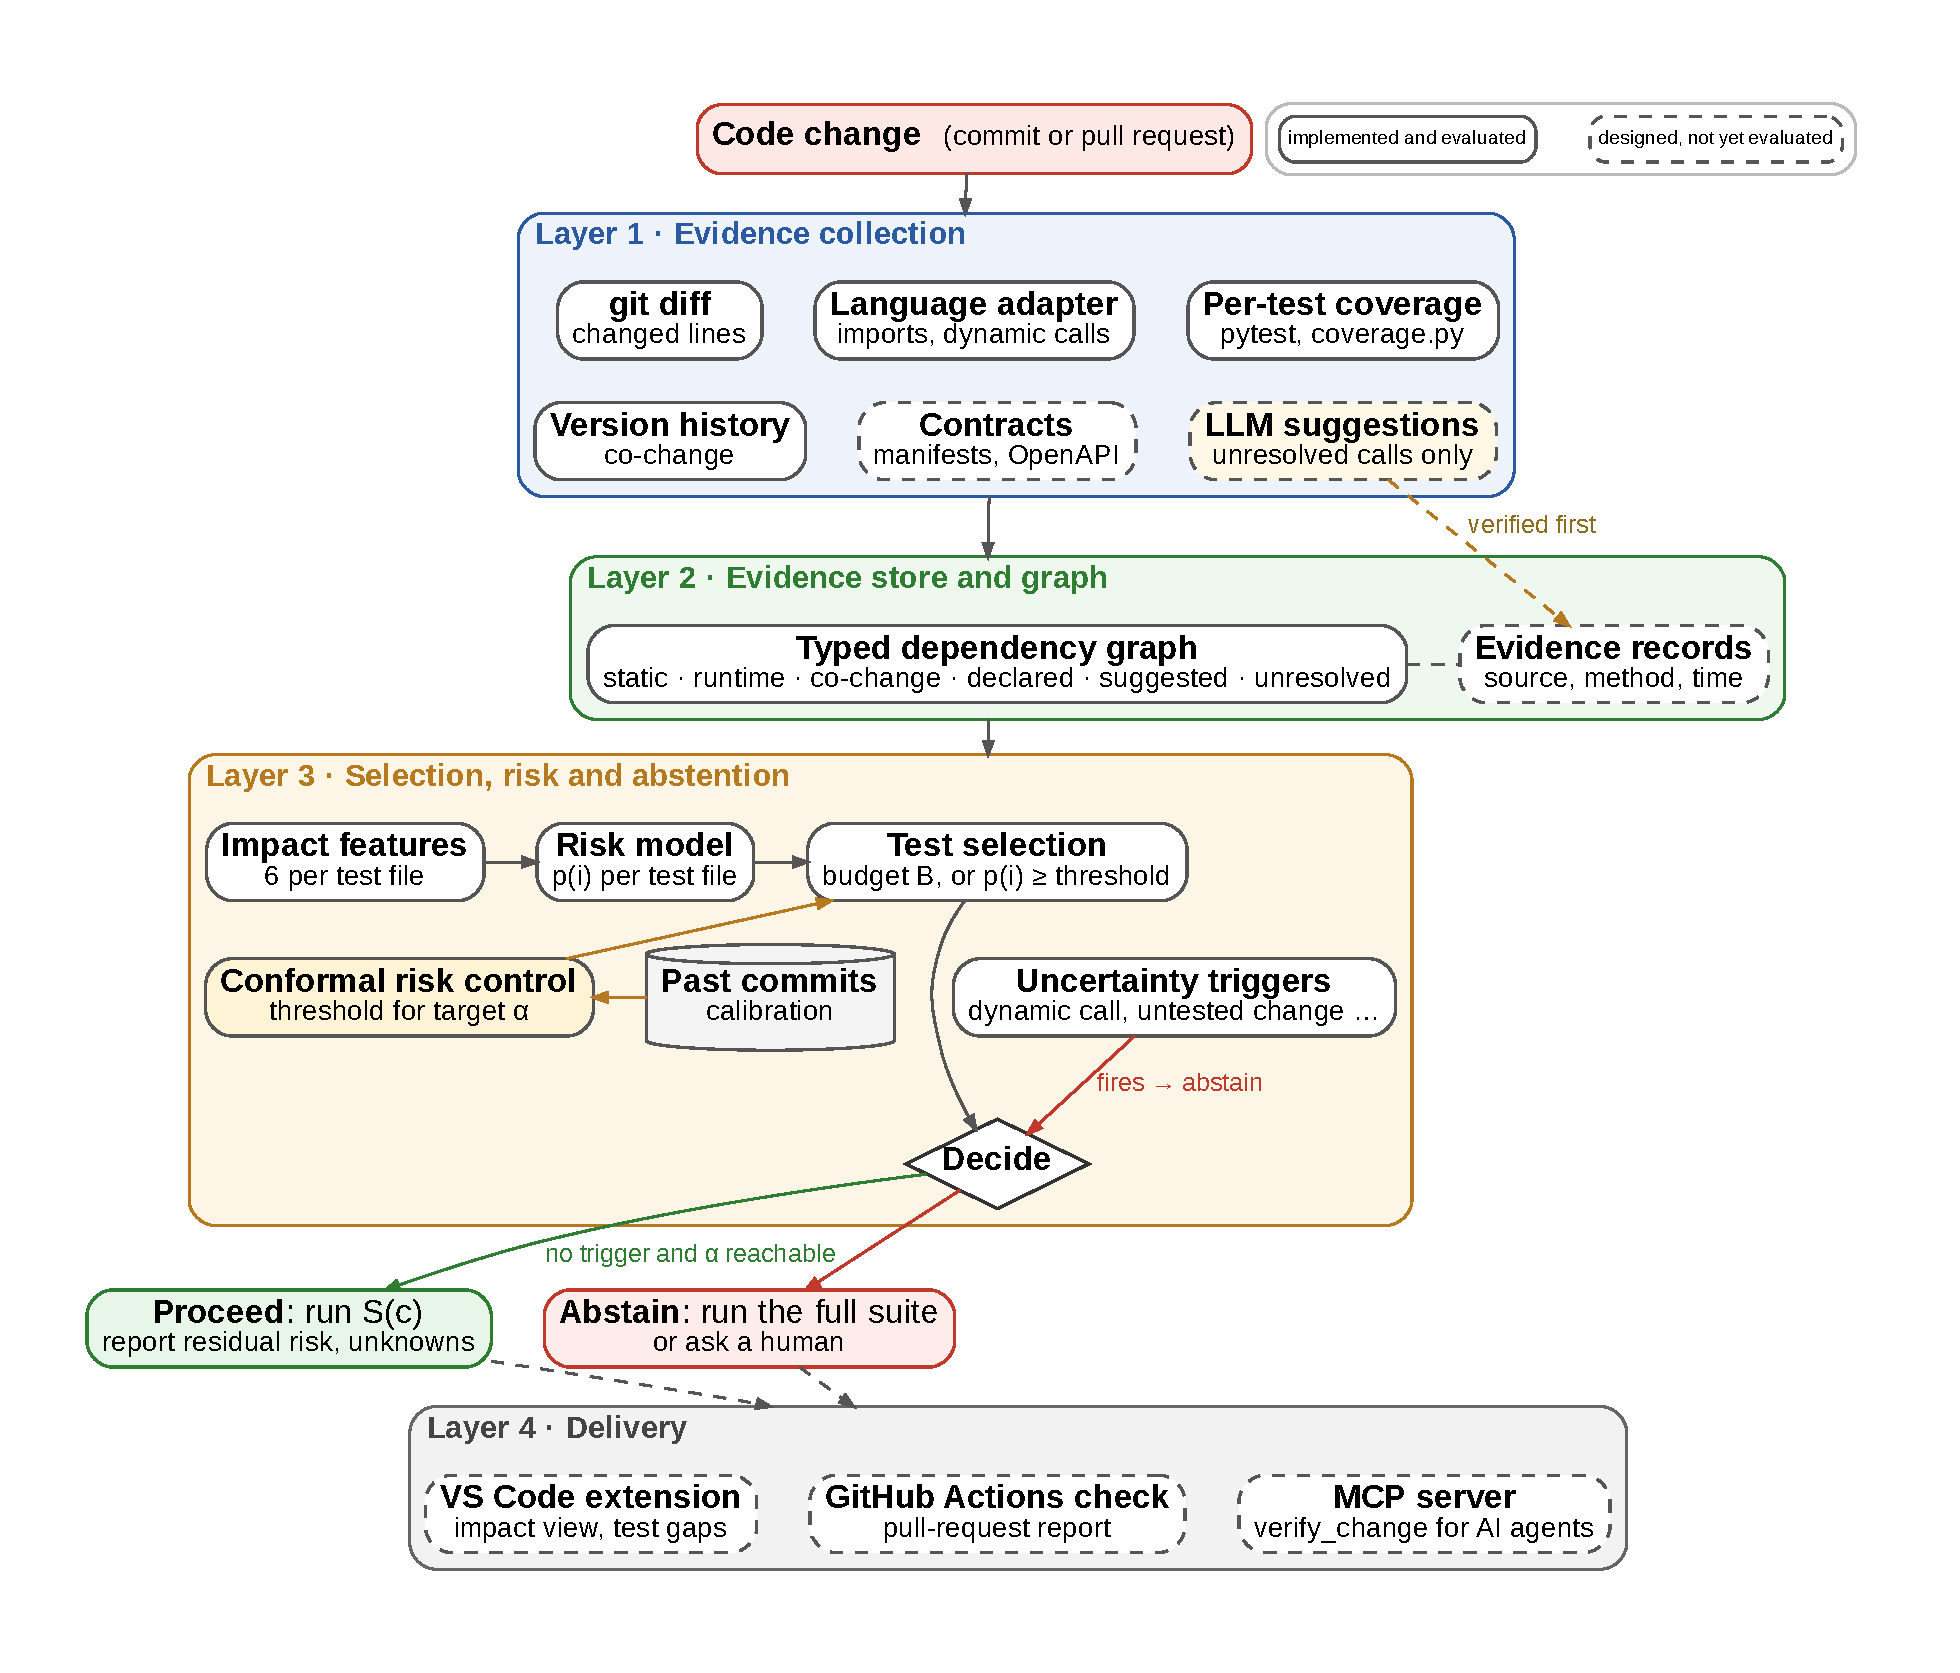
\includegraphics[width=0.85\textwidth]{figures/architecture_v2.pdf}}
\caption{Architecture and decision flow of CodeTwin AI. Layer~1 collects evidence about a change, and Layer~2 stores it in a typed dependency graph. Layer~3 calculates a score for each test file and selects tests within a budget or above a threshold calibrated on recent commits; if the estimated residual risk is above the target, it abstains to a broader run (rule-based uncertainty triggers are evaluated as an alternative). Layer~4 delivers the decision. Solid boxes have been implemented and evaluated in this paper; dashed boxes have been designed but not evaluated.}
\label{fig:arch}
\end{figure*}

\subsection{Blind-Spot-Aware Evidence Graph}
The nodes in the graph represent files, functions, classes, tests, API endpoints and configuration keys. Each edge has one type of evidence: \emph{static} (found in the syntax tree), \emph{runtime-observed} (recorded by per-test coverage), \emph{declared} (taken from a manifest or API contract), \emph{co-change} (files that repeatedly change together in the version history), \emph{suggested} (proposed by a language model but not yet verified) or \emph{unresolved}, an edge that the analysis knows exists but could not resolve, for example a \texttt{getattr} call with a computed name. Each record stores where it came from, the tool that generated it and a timestamp, which allows old evidence to be recognised. Unresolved edges are stored and counted, so the report shows what the analysis could not see instead of treating it as ``no dependency''. In Fig.~\ref{fig:example}, for example, the four dependants of the renamed field are connected by four different evidence types. Every link can be shown to the user as an \emph{evidence card}: the claim, its source file, line and commit, the method that produced it, the time it was generated, the tool version used, and whether it is verified, inferred or unknown.

The prototype also stores three line-level facts for every version of every source file: the span of every function (including its decorators), the lines that contain a dynamic call (\texttt{eval}, \texttt{exec}, \texttt{\_\_import\_\_}, \texttt{import\_module}, or \texttt{getattr}/\texttt{setattr}/\texttt{hasattr} with a computed name), and the lines of statements executed at import time (module-level and class-level statements other than imports, docstrings and simple constants, and all decorators). From this evidence it calculates seven features for every pair of a change and a test file $i$. The features use only the coverage of the previous version and the static facts and diff of the new version: (1)~$x_{\mathit{line}}$, whether $i$ executed a changed line; (2)~$x_{\mathit{func}}$, whether $i$ executed the body of a function that encloses a changed line or insertion point; (3)~$x_{\mathit{file}}$, whether $i$ executed any changed file; (4)~$x_{\mathit{imp}}=1/d$, where $d$ is the import distance from $i$ to a changed module (depth at most six; $0$ if unreachable); (5)~$x_{\mathit{name}}$, whether the name of $i$ contains the name of a changed module; (6)~$x_{\mathit{co}}$, the proportion of the last 300 commits touching the changed files that also touched $i$; and (7)~$x_{\mathit{chg}}$, whether $i$ itself was added or changed.

The changed lines come from a zero-context \texttt{git diff} between the evaluated parent and the change. The coverage of the parent is matched against the \emph{old} line numbers, so no information from running the tests of the change is used. Lines that coverage.py records outside any test context are considered import-time lines. The import graph is built from every \texttt{import} and \texttt{from}\ldots\texttt{import} statement; relative imports are resolved against the package path.

\subsection{Budgeted, Risk-Ranked Selection}\label{sec:select}
A logistic regression model with balanced class weights predicts the likelihood that test file $i$ is affected:
\begin{equation}
p(i) = \sigma\!\left(\mathbf{w}^{\top}\mathbf{x}_i + b\right), \label{eq:model}
\end{equation}
where $\mathbf{x}_i$ is the feature vector above and $\sigma$ the logistic function. In budget mode (Algorithm~\ref{alg:select}, lines 1--7), the tests in $F(c)$ are selected first. The remaining tests are selected in descending order of $p(i)/t(i)$, so the tests with the highest risk per second are selected first, as long as the budget allows. This is the classic greedy approach to the knapsack problem, where the value of a test is the probability that it is affected and its weight is its run time. In calibrated mode (lines 8--14), every test with $p(i)\ge\hat\lambda_c$ is selected, where $\hat\lambda_c$ is a calibrated threshold (Section~\ref{sec:crc}), unless the system abstains. Logistic regression was chosen because the training data are small, its weights can be examined (Section~\ref{sec:ablation}), and its scores increase monotonically with each feature.

\begin{algorithm}[t]
\caption{Risk-ranked selection with calibrated abstention}
\label{alg:select}
\begin{algorithmic}[1]
\Require tests $T$, forced tests $F$, scores $p(i)$, times $t(i)$, budget $B$, target $\alpha$, level $\alpha_c$, recent changes $\mathcal{C}$
\Ensure selected tests $S$, decision $d$
\Statex \textit{Budget mode}
\State $S \gets F$;\ $u \gets \sum_{i\in F} t(i)$
\For{$i \in T\setminus F$ in decreasing order of $p(i)/t(i)$}
  \If{$u + t(i) \le B$}
    \State $S \gets S \cup \{i\}$;\ $u \gets u + t(i)$
  \EndIf
\EndFor
\State \Return $S$
\Statex \textit{Calibrated mode}
\State $\hat\lambda_c \gets$ CRC threshold on $\mathcal{C}$ at level $\alpha_c$ \Comment{Eq.~(\ref{eq:crc})}
\State $S \gets F \cup \{\, i \in T : p(i) \ge \hat\lambda_c \,\}$
\If{$r(c) > \alpha$} \Comment{Eq.~(\ref{eq:rc})}
  \State \Return $S \cup S_{\mathit{broad}}$, \textsc{Abstain} \Comment{broader run}
\EndIf
\State \Return $S$, \textsc{Proceed}
\Statex \textit{After the change's tests run:} $\alpha_{c+1} \gets \alpha_c + \gamma(\alpha - \mathit{err}_c)$
\end{algorithmic}
\end{algorithm}

\subsection{Calibrated Selection Under Drift}\label{sec:crc}
The threshold is chosen using conformal risk control~\cite{angelopoulos2024crc}. Only other projects are used to train the risk model. For a set $\mathcal{C}$ of $n$ earlier changes of the same project and a candidate threshold $\lambda$, the loss for change $c_j$ is one if some affected test outside $F(c_j)$ would be excluded:
\begin{equation}
L_j(\lambda) = \mathbf{1}\big\{\exists\, i \in A(c_j)\setminus F(c_j) : p(i) < \lambda\big\}, \label{eq:loss}
\end{equation}
and the empirical risk is $\hat R_n(\lambda) = \tfrac{1}{n}\sum_{j=1}^{n} L_j(\lambda)$. As the loss is bounded between zero and one and does not decrease as $\lambda$ grows, the threshold
\begin{equation}
\hat\lambda = \sup\Big\{\lambda : \tfrac{n}{n+1}\hat R_n(\lambda) + \tfrac{1}{n+1} \le \alpha\Big\} \label{eq:crc}
\end{equation}
keeps the expected miss rate at or below $\alpha$ when the changes are exchangeable~\cite{angelopoulos2024crc}. The candidate thresholds are the minimum scores of affected tests on the calibration changes, plus $0$ and $1$, so the supremum can be found exactly. If no $\lambda$ qualifies, which happens whenever $\alpha < 1/(n+1)$, every test is selected.

Commits are ordered in time, and projects change: tests are reorganised, modules are split, and the scores shift. We therefore compare three methods for choosing $\mathcal{C}$ and the level. \emph{Static} calibration uses the first 40\% of a project's changes once, as in a preliminary pilot run of this project (results not shown). \emph{Sliding-window} calibration recalculates $\hat\lambda$ for every change from the $n$ most recent earlier changes, where $n$ is the size of the static calibration set. \emph{Adaptive} calibration also uses adaptive conformal inference (ACI)~\cite{gibbs2021aci}: once the tests of change $c$ have run, the level is updated as
\begin{equation}
\alpha_{c+1} = \alpha_c + \gamma\,(\alpha - \mathit{err}_c), \label{eq:aci}
\end{equation}
where $\mathit{err}_c\in\{0,1\}$ records whether the selection missed an affected test and $\gamma=0.02$. A miss lowers the level applied to later changes, which increases their selection; a run of safe changes gradually raises the level again. For ACI, the average miss rate over a long run of changes converges to $\alpha$ without any assumption on how the data shift~\cite{gibbs2021aci}. Both time-aware methods need the true outcome of earlier changes, which can be obtained from post-submit runs, such as Google's periodic milestone runs of affected tests~\cite{memon2017taming} or Meta's full runs on the master branch every few hours~\cite{machalica2019pts}.

\subsection{Residual Risk and Abstention}\label{sec:risk}
For a single change, CodeTwin AI estimates the probability of missing an affected test. First, the model scores of the calibration changes are recalibrated using isotonic regression~\cite{zadrozny2002calibration}, which maps a score to the observed frequency of affected tests, giving $\tilde p(i)$. Assuming independence between skipped tests,
\begin{equation}
r(c) = 1 - \textstyle\prod_{i \in T\setminus S(c)} \big(1-\tilde p(i)\big). \label{eq:rc}
\end{equation}
The system abstains when $r(c)$ is above the target $\alpha$. For the broader run there are three options: the full suite, file-coverage selection (all tests that executed a changed file) and the hybrid of static reachability and file coverage, each combined with the calibrated selection. The rule-based uncertainty triggers of the design were also evaluated (Table~\ref{tab:triggers}). The prototype implements the four triggers that need only single-repository evidence in two forms: \emph{file-level}, as in the pilot run, where a trigger fires if any changed file contains a dynamic call, any changed line ran at import time, and so on; and \emph{line-level}, where only the changed lines and the functions that contain them are counted. The line-level module trigger uses the static import-time statements of the new version instead of the new test run.

\begin{table}[t]
\caption{Uncertainty Triggers}
\label{tab:triggers}
\centering
\footnotesize
\setlength{\tabcolsep}{3pt}
\begin{tabular}{@{}>{\raggedright\arraybackslash}p{0.24\columnwidth}>{\raggedright\arraybackslash}p{0.56\columnwidth}>{\raggedright\arraybackslash}p{0.13\columnwidth}@{}}
\toprule
\textbf{Trigger} & \textbf{Fires when (line-level form)} & \textbf{Status} \\
\midrule
Dynamic call & a changed line, or the function containing it, has a dynamic call & evaluated \\
Untested change & no test executed the function containing a changed line, an edited import-time statement or a new module & evaluated \\
Static/runtime conflict & a test executed a changed line but has no static import path to it & evaluated \\
Module-level change & a changed line is an import-time statement, so all importers are affected & evaluated \\
\midrule
Risk & $r(c) > \alpha$ (Eq.~\ref{eq:rc}) & evaluated \\
\midrule
Unknown consumer & a cross-repository link cannot be resolved & planned \\
Old evidence & coverage or dependency data are older than the code & planned \\
Hidden coupling & files frequently change together but have no code link & planned \\
Unparsable file & there is no adapter, or the changed file cannot be parsed & planned \\
\bottomrule
\end{tabular}
\end{table}

\subsection{Use of Machine Learning and Language Models}
Where static analysis cannot be used, for example at a \texttt{getattr} call with a computed name, a locally run language model is designed to read the surrounding code and suggest likely targets. As language models build less complete call graphs than static tools~\cite{venkatesh2025llmcg}, suggestions are added to the graph only with the type \emph{suggested}. They are promoted to \emph{verified} after a small probe test confirms that the call reaches the proposed target, and they never reduce the risk estimate before that.

The framework is based on one principle: \emph{analysis computes, the model suggests}. Facts about the code are derived from program analysis and test runs; machine learning turns them into a risk estimate (Section~\ref{sec:select}), and statistics checks whether this estimate is honest (Section~\ref{sec:risk}). Besides link suggestion, three other model-based components were designed, each subordinate to evidence. \emph{Retrieval} searches configuration, templates and documentation, other repositories and previous CI logs for dynamic uses of a changed name, and returns each hit with its source. \emph{Targeted test generation} asks a language model to write a test only for a path that no test executes; the test is run before it is accepted, so that the reduction in residual risk can be shown. \emph{Explanation} turns evidence records into readable text and may not add any fact that is not present in a record. Four rules reduce the risk of these components: suggestions remain ``suggested'' until a probe or test confirms them; generated text can only restate what is in the evidence records; the effect of suggestions on the miss rate is measured and reported even if it is negative; and seeds, model and tool versions are recorded alongside the list of evaluated commits. None of these model-based components was implemented or evaluated in this study.

\subsection{Developer and Agent Interfaces}
The design provides the same analysis through three interfaces (Table~\ref{tab:interfaces}). The \emph{VS Code extension} is the main interface: the developer selects code there and can view its impact before making the change. The \emph{GitHub Actions check} runs the same analysis on every pull request and comments on it with the affected components, selected tests, residual risk, unknowns and recommendation. As a \emph{risk-bearing receipt}, it can allow a merge only if the residual risk is below the team's target or a named reviewer has accepted the risk. The \emph{MCP server} allows interaction with AI coding agents: before opening a pull request, an agent can ask whether its change is safe to submit. The agent receives the same calibrated answer as a developer and cannot override it; if CodeTwin AI abstains, the agent is told to run more tests or to ask a human. Current support for agents provides a fixed mapping between code and tests~\cite{alonso2026tdad}; the MCP server adds a calibrated go/no-go decision while using the same engine. These interfaces were not part of the evaluated prototype, and GitHub Actions was used only to run the experiments (Section~\ref{sec:impl}). An initial version of the select-to-impact panel, the MCP tools in Table~\ref{tab:interfaces} and a GitHub Actions step that reports the selection and its risk have since been implemented in the CodeTwin AI tool (release 0.1.0), but they are not evaluated in this paper. The pull-request comment and the risk-bearing receipt have not been implemented yet.

\begin{table}[t]
\caption{Planned Developer and Agent Interfaces}
\label{tab:interfaces}
\centering
\footnotesize
\setlength{\tabcolsep}{3pt}
\begin{tabular}{@{}>{\raggedright\arraybackslash}p{0.33\columnwidth}>{\raggedright\arraybackslash}p{0.62\columnwidth}@{}}
\toprule
\textbf{Feature} & \textbf{What the user receives} \\
\midrule
\multicolumn{2}{@{}l}{\textit{VS Code extension}} \\
Select-to-impact & a side panel with callers, callees, tests and consumers of the selected code; line style shows the evidence type, dotted lines show unresolved links \\
Impact CodeLens & a line above each function, e.g.\ ``used by 7 $\cdot$ 2 repos $\cdot$ 5 tests $\cdot$ 1 unknown'' \\
Blind-spot highlighting & shading of \texttt{getattr}, \texttt{importlib} and \texttt{eval} lines that the analysis cannot follow \\
Test-gap gutter & marking of changed lines that no test executes \\
Recommended tests & ranked tests, budget and residual risk; can be run from the Test Explorer \\
\midrule
\multicolumn{2}{@{}l}{\textit{GitHub Actions pull-request check}} \\
Pull-request report & affected components, selected tests, residual risk, unknowns and recommendation \\
Risk-bearing receipt & merge allowed only below the target risk or with a reviewer's sign-off \\
\midrule
\multicolumn{2}{@{}l}{\textit{MCP server for AI coding agents}} \\
\texttt{verify\_change} & affected components, tests, residual risk, unknowns and a decision: proceed, run\_more or ask\_human \\
\texttt{get\_impact} & the impact map of a symbol or file with the evidence type of every link \\
\texttt{recommend\_tests} & ranked tests within a given budget, each with its reason \\
\texttt{explain\_decision} & the evidence records behind a recommendation \\
\bottomrule
\end{tabular}
\end{table}

\subsection{Planned Extensions}
The same principle applies to further features, planned after the core is evaluated: a model or heuristic suggests, evidence confirms, risk is calibrated and the tool abstains when it is uncertain. \emph{Active link verification} runs a small probe for the uncertain links whose confirmation would lower the residual risk most. An \emph{evidence freshness meter} raises the risk as coverage and dependency data age. A \emph{consumer-evidence contract check} links every API or schema change to consumer code and tests in other repositories, and a \emph{cross-repository collision radar} warns when open pull requests in different repositories have overlapping impact. A \emph{flaky-evidence discount} treats a pass from a flaky test as weaker evidence. In the same way, a \emph{covered-but-unchecked discount} weakens the evidence of a test that executes changed code but survives an extreme mutant of it, a \emph{same-change test rule} trusts a test written together with the change only if it fails on the base commit, and \emph{non-code evidence} records which libraries, configuration keys, environment variables and data files each test reads, so that a dependency or configuration change selects only those tests and an input that no test reads counts as unknown. A \emph{conformal culprit set} reports, for a failing test, the small set of commits that contains the cause with a chosen confidence, and a \emph{promise monitor} tracks the observed miss rate against the promised target over time and alerts on drift.

% =====================================================================
\section{Implementation}\label{sec:impl}
% =====================================================================
The prototype consists of three Python scripts. The \emph{collector} (532 lines) checks out each evaluated change and its parent and captures the diff. It collects the static facts of every file with the Python \texttt{ast} module and runs the test suite with pytest~8, pytest-cov and coverage.py (C tracer, one coverage context per test) to obtain per-test-file coverage, run times and per-test-case outcomes. It then seeds up to three faults on the changed lines of the new version (Section~\ref{sec:gt}) and runs the test files that executed the mutated file; each test has a timeout, so a test that hangs counts as failing. The \emph{analysis} script (909 lines) calculates the ground truths, baselines, risk model (scikit-learn logistic regression and isotonic regression), the three calibration variants, residual risk, triggers, abstention, ablation, bootstrap confidence intervals and paired tests with SciPy. A third script writes every number in this paper from the analysis output, so no result was typed manually.

The experiments were run on GitHub Actions with Python~3.12. One workflow splits each project's changes into contiguous shards, and 52 collection jobs run in parallel on Ubuntu runners; a final job combines the data and runs the analysis. The list of commits is fixed by a cutoff date (10 November 2026), so a rerun selects the same changes. For the NameRTS projects we installed each project's test dependencies once from its latest commit, and fixed the pandas and NumPy versions of the NameRTS replication environment so that older commits can still be run. After the study, the evidence store (SQLite), an initial VS Code extension, a GitHub Actions step and the MCP server were implemented in the CodeTwin AI tool (release 0.1.0). They use the same scoring, calibration and abstention code but were not used in these experiments. The language-model link suggestions, the pull-request comment and receipt, cross-repository evidence and adapters for other languages have not been implemented yet. The prototype, the scripts and the manuscript text were prepared with the assistance of Claude Opus 5.5 (Anthropic); the authors conceived the approach and reviewed all code and text (see the AI-use statement at the end of the paper).

% =====================================================================
\section{Experimental Setup}\label{sec:setup}
% =====================================================================
\subsection{Research Questions}
We answer the research question in the Introduction through four research questions that test the hypotheses H1 to H3; a fourth hypothesis, on verified language-model suggestions (H4), is left for future work.

\textbf{RQ1 (selection quality, H1).} At the same time budget, does risk-ranked selection find more affected tests than simpler baselines? A time-saving method is only useful if it still finds the tests that a change can break.

\textbf{RQ2 (calibration, H2).} Does the observed miss rate on later changes stay at or below the target $\alpha$, and does the per-change estimate $r(c)$ match how often selections actually miss? This ensures that the stated risk can be trusted on changes the system has not seen.

\textbf{RQ3 (abstention, H3).} Can uncertainty triggers and risk-based abstention flag the changes on which conventional selection misses tests, with an acceptable abstention rate and cost?

\textbf{RQ4 (faults and NameRTS).} Do the selections detect seeded faults, and how does CodeTwin AI compare with NameRTS on NameRTS's own changes and ground truth?

\subsection{Subject Projects}
Table~\ref{tab:subjects} lists the subjects. The five \emph{history} projects (click, python-dateutil, itsdangerous, marshmallow and toolz) are open-source Python libraries with pytest suites. For each, we took up to the last 250 mainline commits before the cutoff that change at least one source file, and compared each with the previous commit. Merge commits were included, as most changes to these projects are made through pull-request merges. Changes whose old or new version could not be tested with per-test coverage on Python~3.12 were removed (266 changes, mostly old commits of toolz and marshmallow), and dateutil has only 51 source-changing mainline commits since it moved to its current source layout. The 3 \emph{NameRTS} projects use exactly the commit pairs of the NameRTS replication package~\cite{wang2026namerts}: for each target commit, we compare it with the parent used by NameRTS. In total, 681 changes were evaluated, with 332 test changes on the history projects and 79 on the NameRTS projects.

\begin{table}[t]
\caption{Subject Projects}
\label{tab:subjects}
\centering
\footnotesize
\setlength{\tabcolsep}{1.8pt}
\begin{tabular}{@{}lrrrrrrr@{}}
\toprule
\textbf{Project} & \textbf{Changes} & \textbf{KLoC} & \textbf{Tests} & \textbf{Suite} & \textbf{Aff.} & \textbf{Mut.} & \textbf{Years} \\
\midrule
click & 250 (100/150) & 12.9 & 22 & 2.3 & 10.7 & 353 & 2020--2026 \\
dateutil & 51 (20/31) & 8.5 & 16 & 31.6 & 7.1 & 68 & 2022--2026 \\
itsdangerous & 50 (20/30) & 1.2 & 5 & 1.2 & 1.9 & 27 & 2018--2025 \\
marshmallow & 149 (59/90) & 5.0 & 12 & 1.9 & 5.6 & 99 & 2021--2026 \\
toolz & 51 (20/31) & 3.8 & 11 & 0.3 & 3.0 & 48 & 2013--2026 \\
\midrule
loguru$^\ast$ & 38 (15/23) & 5.6 & 49 & 121.3 & 27.3 & 65 & 2023--2025 \\
pvlib$^\ast$ & 45 (18/27) & 35.3 & 55 & 78.0 & 4.4 & 69 & 2025 \\
seaborn$^\ast$ & 47 (18/29) & 29.3 & 34 & 350.0 & 8.1 & 83 & 2023--2025 \\
\bottomrule
\multicolumn{8}{@{}p{0.97\columnwidth}@{}}{Changes = evaluated changes (calibration/test); Tests = mean test files; Suite = mean full-suite time with coverage (s); Aff.\ = mean affected test files per change; Mut.\ = seeded faults detected by at least one test. $^\ast$NameRTS commit pairs.}
\end{tabular}
\end{table}

\subsection{Ground Truths}\label{sec:gt}
\emph{Coverage.} We count a test file as \textit{affected} by a change if, in the new version, (a)~it runs a changed source line (according to per-test coverage contexts); (b)~it runs a module whose import-time code changed; (c)~the test file itself was added or changed; or (d)~in the old version, it ran a source file that the change deleted. Coverage tells us which tests could notice a change. It does not tell us which tests would fail.

\emph{Seeded faults.} To measure fault detection, we seeded up to three mutants per change. Each mutant sits on a different, randomly chosen changed line of the new version and uses one of nine classic operators~\cite{jia2011mutation}: relational, arithmetic and logical operator replacement, negation removal, Boolean and integer constant replacement, return-value replacement, call-statement deletion and assignment-value replacement. A test file \emph{detects} a mutant when one of its test cases passed on the unmutated code but fails on the mutant. We run each mutant only against the test files that executed the mutated file. We drop mutants that no test detects (survivors, which include equivalent mutants) and mutants whose run timed out or did not start. Mutant detection is known to correlate with the detection of real faults~\cite{just2014mutants}.

\emph{NameRTS.} For the NameRTS projects we also use the ground truth of affected test files published with NameRTS~\cite{wang2026namerts}, limited to the test files that exist in our runs.

\subsection{Baselines}
\textit{Retest-all} runs every test file. \textit{Name matching} picks the test files whose name contains the name of a changed module; this simple heuristic is inspired by NameRTS~\cite{wang2026namerts}. \textit{Static import} picks the test files that reach a changed module through the import graph, as static class- or file-level RTS does~\cite{legunsen2016static}. \textit{File coverage} picks the tests that executed a changed file in the previous version, in the style of Ekstazi~\cite{gligoric2015ekstazi}. \textit{Function coverage} and \textit{Line coverage} are stricter: the test must have executed a changed function or a changed line. \textit{Hybrid} is the union of static import and file coverage. All baselines also run the test files that the change adds or modifies. For the time-budget experiments, \textit{Random} orders the test files at random (20 seeds), and \textit{Coverage-ranked} orders them by a fixed weighted sum of the coverage and import features. On the NameRTS projects we also evaluate the \textit{published NameRTS selections}, so we compare against NameRTS itself rather than our own re-implementation of it.

\subsection{Metrics}
With $T$, $t(i)$, $A(c)$ and $S(c)$ defined as before, we report four measures per change and average them over changes: test reduction $1-|S|/|T|$, time reduction $1-\sum_{i\in S}t(i)/\sum_{i\in T}t(i)$, precision $|S\cap A|/|S|$ and recall $|S\cap A|/|A|$. Precision and recall are averaged only over changes with at least one affected test. A selection is \textit{safe} for a change if $A(c)\subseteq S(c)$, and the observed miss rate is the share of changes on which it is unsafe. For seeded faults we report the \textit{mutant detection rate}: of the mutants that some test detects, the share for which the selection keeps at least one detecting test. To judge $r(c)$ we use the Brier score~\cite{brier1950verification}, the mean squared difference between $r(c)$ and the observed miss (0 or 1), and compare it with the score of a constant forecast; we also report the expected calibration error over five bins. Run times are those measured on the new version.

\subsection{Protocol}
Fig.~\ref{fig:workflow} gives an overview of the study. The changes of each project are put in time order. The first 40\% are used for calibration and the rest are test changes; calibration changes are never used for training. We train the risk model leave-one-project-out on the other history projects, and use a model trained on all history projects for the NameRTS projects. Budgets are 10\%, 25\% and 50\% of the full-suite time of the previous version, and the targets are $\alpha\in\{0.01,0.05,0.10,0.20\}$. The sliding window and ACI start from the same calibration set, and ACI uses $\gamma=0.02$, which we fixed in advance. The isotonic recalibration for $r(c)$ is fitted on the calibration changes. For the ablation we retrain the model without one evidence signal, or without all coverage signals, and compare the variants at the 25\% budget. We report 95\% bootstrap confidence intervals (10,000 resamples over test changes) and paired Wilcoxon signed-rank tests for recall.

% =====================================================================

\begin{figure*}[t]
\centering
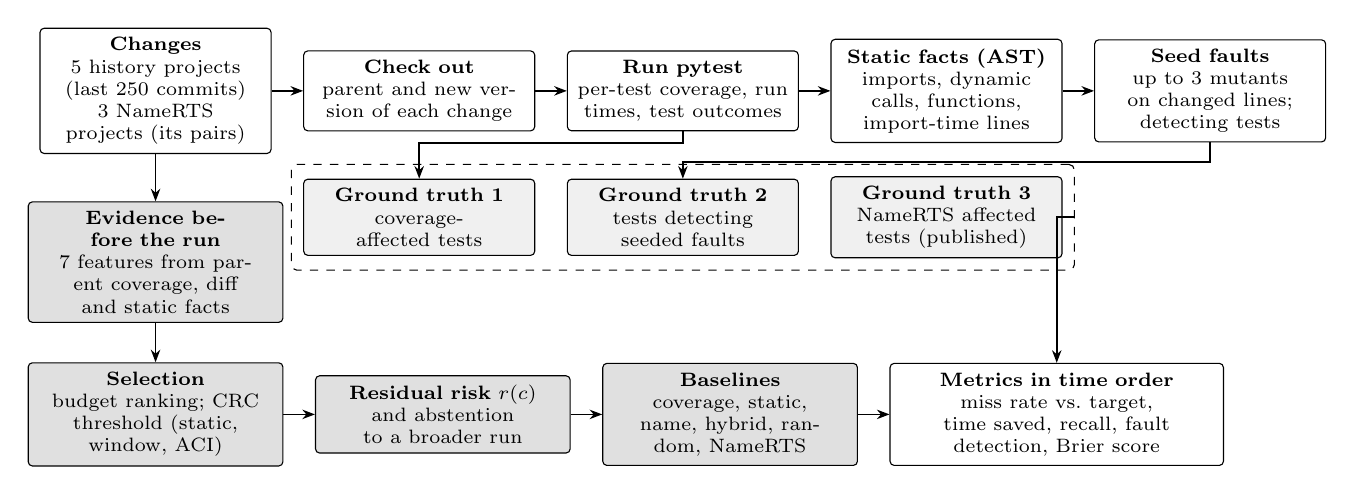
\begin{tikzpicture}[font=\scriptsize, node distance=3.5mm and 4mm,
  box/.style={draw, rounded corners=1.5pt, align=center, minimum height=9mm, text width=27mm, fill=white},
  gt/.style={box, fill=black!6}, an/.style={box, text width=30mm, fill=black!12},
  arr/.style={-{Stealth[length=1.6mm]}, semithick}]
\node[box] (hist) {\textbf{Changes}\\ 5 history projects (last 250 commits)\\ 3 NameRTS projects (its pairs)};
\node[box, right=of hist] (co) {\textbf{Check out}\\ parent and new version of each change};
\node[box, right=of co] (run) {\textbf{Run pytest}\\ per-test coverage, run times, test outcomes};
\node[box, right=of run] (st) {\textbf{Static facts (AST)}\\ imports, dynamic calls, functions, import-time lines};
\node[box, right=of st] (mut) {\textbf{Seed faults}\\ up to 3 mutants on changed lines; detecting tests};
\node[gt, below=6mm of co] (g1) {\textbf{Ground truth 1}\\ coverage-affected tests};
\node[gt, right=of g1] (g2) {\textbf{Ground truth 2}\\ tests detecting seeded faults};
\node[gt, right=of g2] (g3) {\textbf{Ground truth 3}\\ NameRTS affected tests (published)};
\node[an, below=6mm of hist] (f) {\textbf{Evidence before the run}\\ 7 features from parent coverage, diff and static facts};
\node[an, below=5mm of f] (sel) {\textbf{Selection}\\ budget ranking; CRC threshold (static, window, ACI)};
\node[an, right=of sel] (risk) {\textbf{Residual risk} $r(c)$\\ and abstention to a broader run};
\node[an, right=of risk] (base) {\textbf{Baselines}\\ coverage, static, name, hybrid, random, NameRTS};
\node[box, right=of base, text width=40mm] (met) {\textbf{Metrics in time order}\\ miss rate vs.\ target, time saved, recall, fault detection, Brier score};
\draw[arr] (hist) -- (co); \draw[arr] (co) -- (run); \draw[arr] (run) -- (st); \draw[arr] (st) -- (mut);
\draw[arr] (run.south) -- ++(0,-1.5mm) -| (g1.north);
\draw[arr] (mut.south) |- ++(0,-2.5mm) -| (g2.north);
\draw[arr] (hist.south) -- (f.north);
\draw[arr] (f) -- (sel); \draw[arr] (sel) -- (risk); \draw[arr] (risk) -- (base); \draw[arr] (base) -- (met);
\node[draw, dashed, rounded corners=2pt, inner sep=1.5mm, fit=(g1)(g2)(g3)] (gts) {};
\draw[arr] (gts.east) -| (met.north);
\end{tikzpicture}
\caption{Study workflow. The collection steps (top row) run on GitHub Actions in 52 parallel shards. The analysis (bottom row) processes each project's changes in time order and uses the test run of the new version only to build the ground truths.}
\label{fig:workflow}
\end{figure*}
\section{Results}\label{sec:results}
% =====================================================================
\subsection{RQ1: Selection Quality}
Table~\ref{tab:rq1} compares all techniques on the 332 test changes of the history projects. The baselines show a clear trade-off. File coverage and the hybrid never missed an affected test, but they saved only 26.5\% and 9.0\% of test time. Function and line coverage saved more (41.4\% and 43.3\%) but were unsafe on 17.2\% and 9.3\% of changes. Name matching saved the most time (75.2\%), but its recall was only 0.39. We expected function coverage to fix the misses of line coverage, yet it was less safe. The reason is that a function's signature and decorators run at import time. When a change edits them, line coverage keeps every test that loaded the module, while function coverage keeps only the tests that ran the function body.

\begin{table}[t]
\caption{Selection Quality on the History Projects (Mean Over 332 Test Changes)}
\label{tab:rq1}
\centering
\footnotesize
\setlength{\tabcolsep}{1.6pt}
\begin{tabular}{@{}lrrrrrr@{}}
\toprule
\textbf{Technique} & \textbf{TestR\%} & \textbf{TimeR\%} & \textbf{Prec.} & \textbf{Rec.} & \textbf{Safe\%} & \textbf{Mut.\%} \\
\midrule
Retest-all & 0.0 & 0.0 & 0.54 & 1.00 & 100.0 & 100.0 \\
Name matching & 85.4 & 75.2 & 0.91 & 0.39 & 28.6 & 87.5 \\
Static import & 17.9 & 11.1 & 0.62 & 0.97 & 96.4 & 99.7 \\
File coverage & 36.5 & 26.5 & 0.80 & 1.00 & 100.0 & 99.7 \\
Function coverage & 53.6 & 41.4 & 0.91 & 0.90 & 82.8 & 99.7 \\
Line coverage & 54.6 & 43.3 & 0.97 & 0.93 & 90.7 & 99.7 \\
Hybrid (static $\cup$ file cov.) & 15.7 & 9.0 & 0.62 & 1.00 & 100.0 & 99.7 \\
\midrule
CodeTwin, budget 25\% & 46.9 & 72.0 & 0.66 & 0.65 & 34.6 & 91.1 \\
CodeTwin, ACI $\alpha$=0.1 & 49.9 & 39.1 & 0.90 & 0.94 & 90.7 & 99.7 \\
\quad + risk abstention & 39.7 & 29.7 & 0.83 & 0.99 & 98.2 & 99.7 \\
\bottomrule
\multicolumn{7}{@{}p{0.97\columnwidth}@{}}{Mut.\% = share of detected seeded faults for which the selection contains a detecting test.}
\end{tabular}
\end{table}

Fig.~\ref{fig:budget} shows the results in budget mode. With 10, 25 and 50\% of the full-suite time, the learned ranking reached a recall of 0.490, 0.655 and 0.815. It did better than random selection at every budget (paired Wilcoxon tests, $p<10^{-4}$, $p<10^{-4}$ and $p<10^{-4}$; mean differences +0.055, +0.075 and +0.061), but it was practically the same as the coverage ranking (0.490, 0.654 and 0.811; $p=0.89$, $p=0.18$ and $p=0.26$). Even with half of the suite's time, at most 37.0\% of changes were safe. A fixed budget therefore cannot promise safety, which is why a calibrated mode is needed.

Fig.~\ref{fig:tradeoff} plots every technique by time saved and miss rate. On these projects the coverage baselines form the frontier. Adaptive calibration moves along this frontier as the target changes, and risk-based abstention sits just above file coverage: it saves slightly more time at the cost of a small miss rate.

\begin{figure}[t]
\centering
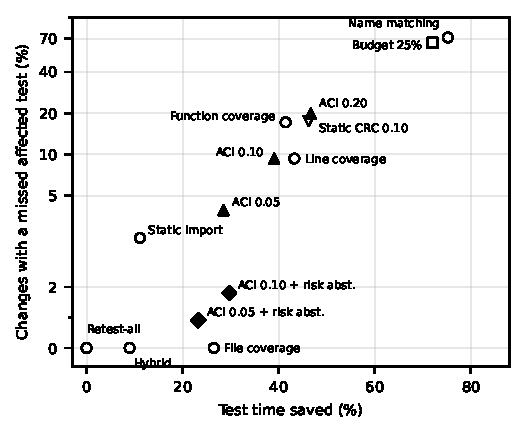
\includegraphics[width=\columnwidth]{figures/tradeoff.pdf}
\caption{Time saved against the share of changes with a missed affected test (history projects; vertical axis linear up to 5\%, then logarithmic). Circles: baselines; triangles: CodeTwin AI with adaptive calibration; diamonds: with risk-based abstention.}
\label{fig:tradeoff}
\end{figure}

\textbf{Answer to RQ1:} within the same budget, risk-ranked selection finds more affected tests than random selection, but on these projects it adds nothing over a coverage ranking (H1 is not supported against coverage-only selection).

\begin{figure}[t]
\centering
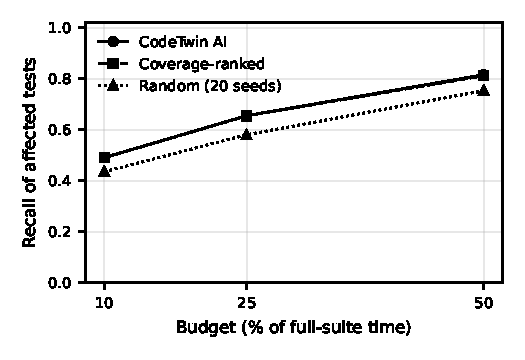
\includegraphics[width=\columnwidth]{figures/budget.pdf}
\caption{Recall of affected tests at different time budgets (history projects).}
\label{fig:budget}
\end{figure}

\subsection{RQ2: Calibration and Residual Risk}
Table~\ref{tab:rq2} and Fig.~\ref{fig:calib} give the observed miss rate for each target. Static calibration, fitted once on the oldest 40\% of each project's changes, did not hold. For targets of 5\%, 10\% and 20\%, it missed affected tests on 11.4\%, 17.5\% and 28.0\% of later changes. The worst case was marshmallow: the threshold fitted on old changes (0.978) was too high for the newer ones, and 26.7\% of test changes were missed. The sliding window, which recalibrates on recent changes, came closer (5.7\%, 12.0\% and 21.1\%). Adaptive calibration kept the miss rate at or below every target on the history projects: 0.6\%, 4.5\%, 9.3\% and 19.9\% for targets of 1\%, 5\%, 10\% and 20\%. At the three larger targets it saved 28.5\%, 39.1\% and 46.7\% of test time. At $\alpha=0.10$ it was as safe as line coverage (90.7\%) and saved slightly less time. The difference is that its level is chosen in advance and can be tightened: at $\alpha=0.05$ it was safe on 95.5\% of changes. The pooled numbers hide some variation (Fig.~\ref{fig:perproject}). Per history project, adaptive calibration at $\alpha=0.10$ missed between 6.5\% and 11.1\% of changes (highest for marshmallow), so a single project can exceed the target by about one percentage point; on the NameRTS commits the highest was 13.8\% (seaborn). In the pilot run, with 15--16 calibration changes per project, static calibration seemed valid. With 20--100 calibration changes spread over longer periods, drift dominates.

\begin{table}[t]
\caption{Observed Miss Rate (\%) and Time Saved (\%) per Target $\alpha$ (History Projects)}
\label{tab:rq2}
\centering
\footnotesize
\setlength{\tabcolsep}{3pt}
\begin{tabular}{@{}lrrrrrr@{}}
\toprule
& \multicolumn{2}{c}{\textbf{Static}} & \multicolumn{2}{c}{\textbf{Sliding window}} & \multicolumn{2}{c}{\textbf{Adaptive (ACI)}} \\
\cmidrule(lr){2-3}\cmidrule(lr){4-5}\cmidrule(l){6-7}
$\alpha$ & Miss & Time & Miss & Time & Miss & Time \\
\midrule
0.01 & 1.2 & 9.8 & 0.9 & 9.4 & 0.6 & 7.2 \\
0.05 & 11.4 & 40.5 & 5.7 & 36.0 & 4.5 & 28.5 \\
0.10 & 17.5 & 46.2 & 12.0 & 41.7 & 9.3 & 39.1 \\
0.20 & 28.0 & 50.7 & 21.1 & 47.1 & 19.9 & 46.7 \\
\bottomrule
\end{tabular}
\end{table}

\begin{figure}[t]
\centering
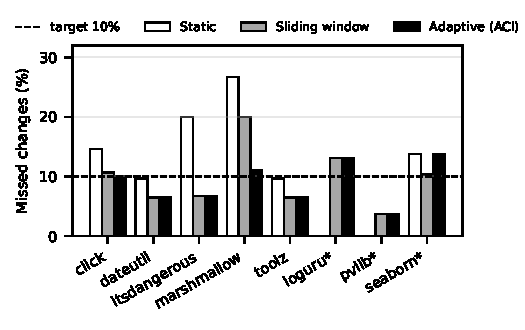
\includegraphics[width=\columnwidth]{figures/per_project.pdf}
\caption{Share of changes with a missed affected test per project at target $\alpha=0.10$ ($^\ast$NameRTS commits). A bar of zero means no miss.}
\label{fig:perproject}
\end{figure}

\begin{figure}[t]
\centering
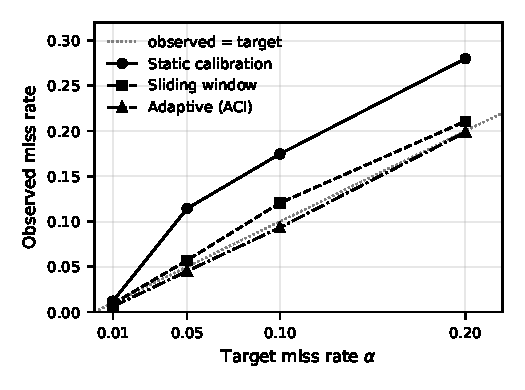
\includegraphics[width=\columnwidth]{figures/calibration.pdf}
\caption{Observed miss rate against the target $\alpha$ for the three calibration variants (history projects). Points below the dotted line meet the target.}
\label{fig:calib}
\end{figure}

The per-change estimate $r(c)$ separated risky selections from safe ones. In budget mode at 25\%, where selections are often unsafe, its mean was 68.3\% against an observed miss rate of 65.4\%, and its Brier score was 0.064 against 0.226 for a constant forecast. For the adaptively calibrated selections at $\alpha=0.10$, it overestimated the risk (mean 12.7\% against 9.3\% observed; Brier score 0.076 against 0.085 for a constant forecast). A likely reason is that skipped tests are not independent, as Eq.~(\ref{eq:rc}) assumes: when one skipped test is affected, others often are too. The estimate still separated changes well. The 265 of 332 changes with $r(c)<0.2$ were missed 3.8\% of the time, and the 11 changes with $r(c)>0.8$ were missed 81.8\% of the time. Fig.~\ref{fig:reliability} shows the reliability diagram. The main value of $r(c)$ is therefore in ranking changes by risk, which RQ3 builds on.

\begin{figure}[t]
\centering
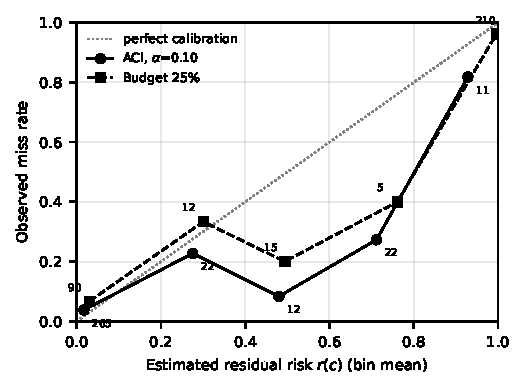
\includegraphics[width=\columnwidth]{figures/reliability.pdf}
\caption{Reliability of the residual-risk estimate $r(c)$ (history projects): mean estimate against observed miss rate in five bins; numbers give the changes per bin. Points below the diagonal overestimate the risk.}
\label{fig:reliability}
\end{figure}

\textbf{Answer to RQ2:} on the history projects, the miss rate stays at the target only when calibration adapts over time (H2 is supported for ACI but not for static calibration). The estimate $r(c)$ ranks changes by risk but overstates how high the risk is for calibrated selections.

\subsection{RQ3: Uncertainty Triggers and Risk-Based Abstention}
Line coverage was unsafe on 31 of the 332 test changes (9.3\%). The file-level triggers of the original design flagged 29 of these changes, but they also fired on 85.7\% of the safe changes. Limiting the triggers to changed lines halved the abstention rate, but they then caught only 7 of the 31 unsafe changes, a smaller share than they flagged among the safe ones (49.2\%). In other words, the line-level rules did not point at the changes that were actually risky. The risk rule $r(c)>\alpha$, applied to the line-coverage selection, flagged 26 of the 31 unsafe changes and fired on only 27.2\% of the safe ones.

Fig.~\ref{fig:triggers} compares the three rules side by side.

\begin{figure}[t]
\centering
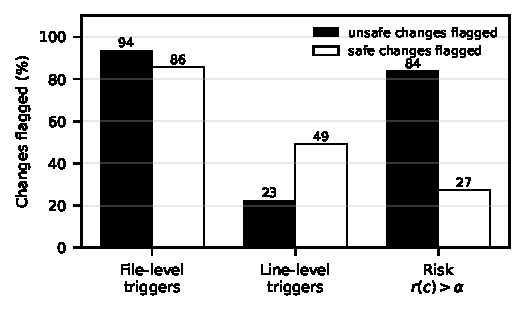
\includegraphics[width=\columnwidth]{figures/triggers.pdf}
\caption{Share of unsafe and of safe changes (for line-coverage selection) that each abstention rule flags (history projects). A useful rule flags many unsafe and few safe changes.}
\label{fig:triggers}
\end{figure}

Table~\ref{tab:rq3} shows what each policy costs on top of adaptive calibration at $\alpha=0.10$. File-level triggers made almost every change safe, but they abstained on 86.4\% of changes, which left a saving of 6.8\% with the full suite as fallback. Risk-based abstention fired on 25.9\% of changes. With file-coverage selection as the broader run, 98.2\% of changes were safe and 29.7\% of test time was saved. At $\alpha=0.05$ the same policy missed 0.9\% of changes and saved 23.3\%. For comparison, file coverage on its own was safe on every change and saved 26.5\%. On these projects, then, abstention does not add savings; what it adds is a stated risk that can be adjusted.

\begin{table}[t]
\caption{Abstention Policies on Top of ACI ($\alpha=0.10$, History Projects)}
\label{tab:rq3}
\centering
\footnotesize
\setlength{\tabcolsep}{2pt}
\begin{tabular}{@{}llrrrr@{}}
\toprule
\textbf{Abstain when} & \textbf{Broader run} & \textbf{Abst.\%} & \textbf{Miss\%} & \textbf{Time\%} & \textbf{Mut.\%} \\
\midrule
File-level triggers & full suite & 86.4 & 0.3 & 6.8 & 100.0 \\
File-level triggers & file coverage & 86.4 & 0.3 & 28.1 & 99.7 \\
File-level triggers & hybrid & 86.4 & 0.3 & 15.1 & 99.7 \\
\midrule
Line-level triggers & full suite & 46.7 & 6.0 & 26.2 & 100.0 \\
Line-level triggers & file coverage & 46.7 & 6.0 & 36.3 & 99.7 \\
Line-level triggers & hybrid & 46.7 & 6.0 & 29.9 & 99.7 \\
\midrule
Risk $r(c)>\alpha$ & full suite & 25.9 & 1.8 & 25.0 & 99.7 \\
Risk $r(c)>\alpha$ & file coverage & 25.9 & 1.8 & 29.7 & 99.7 \\
Risk $r(c)>\alpha$ & hybrid & 25.9 & 1.8 & 25.9 & 99.7 \\
\bottomrule
\end{tabular}
\end{table}

\textbf{Answer to RQ3:} the rule-based triggers either fire on most changes (file level) or miss most of the risky ones (line level). Abstaining on the estimated risk flags most unsafe changes at a moderate abstention rate (H3 is supported for risk-based abstention only).

\subsection{RQ4: Seeded Faults and Comparison With NameRTS}
The tests detected 812 seeded faults in total. For 478 of the 479 detected faults on test changes (99.8\%), every detecting test was inside the coverage-defined affected set, so the coverage ground truth included the tests that matter for these faults. The one exception came from itsdangerous, whose test classes are reused across test files: pytest reported the detecting test under a different file from the one in which coverage recorded it. All coverage-based selections detected 358 of the 359 detected faults of the history projects, name matching detected 314, and the 25\% budget 327 (Table~\ref{tab:rq1}). Detecting the seeded faults was therefore easier than keeping every affected test: a selection that missed affected tests usually still kept a test that detected the fault.

\begin{table}[t]
\caption{NameRTS Commits (79 Test Changes of 3 Projects)}
\label{tab:rq4}
\centering
\footnotesize
\setlength{\tabcolsep}{2pt}
\setlength{\tabcolsep}{3pt}
\begin{tabular}{@{}lrrrr@{}}
\toprule
& & \multicolumn{2}{c}{\textbf{Safe\%}} & \\
\cmidrule(lr){3-4}
\textbf{Technique} & \textbf{Time\%} & \textbf{cov.} & \textbf{NameRTS} & \textbf{Mut.\%} \\
\midrule
Retest-all & 0.0 & 100.0 & 100.0 & 100.0 \\
NameRTS & 68.7 & 62.0 & 100.0 & 99.2 \\
Line coverage & 63.2 & 84.8 & 88.6 & 100.0 \\
Function coverage & 56.7 & 74.7 & 91.1 & 100.0 \\
File coverage & 45.3 & 100.0 & 94.9 & 100.0 \\
Static import & 2.3 & 92.4 & 93.7 & 100.0 \\
Name matching & 84.9 & 34.2 & 44.3 & 99.2 \\
\midrule
CodeTwin, ACI $\alpha$=0.1 & 50.3 & 89.9 & 92.4 & 100.0 \\
\quad + risk abstention & 47.8 & 94.9 & 94.9 & 100.0 \\
CodeTwin, budget 25\% & 75.0 & 41.8 & 55.7 & 95.0 \\
\bottomrule
\multicolumn{5}{@{}p{0.97\columnwidth}@{}}{Safe\% by our coverage ground truth (cov.) and by the published NameRTS ground truth.}
\end{tabular}
\end{table}

Table~\ref{tab:rq4} compares the techniques on the NameRTS commit pairs. NameRTS saved 68.7\% of test time and, by its own ground truth, was safe on every change, which is consistent with its paper~\cite{wang2026namerts}. By our coverage ground truth, however, it was safe on only 62.0\% of changes, and it detected 99.2\% of the seeded faults. The two ground truths disagree because they count different things: coverage counts every test that executes a changed line, whereas NameRTS counts the tests that are reachable through name dependencies. Adaptive calibration at $\alpha=0.10$ was safe on 89.9\% of changes by coverage and on 92.4\% by the NameRTS ground truth, and saved 50.3\%. With risk-based abstention it was safe on 94.9\% of changes (coverage) and saved 47.8\%. Each NameRTS project has only 15--18 calibration changes, too few for static calibration to reach targets of 1\% and 5\%. Adaptive calibration missed 5.1\%, 10.1\% and 21.5\% of changes for targets of 5\%, 10\% and 20\%, which is close to the target but slightly above it on these short histories.

\textbf{Answer to RQ4:} the coverage ground truth contains nearly all tests that detect seeded faults. NameRTS is more efficient, while CodeTwin AI is safer by coverage and states its risk; which of the two is safer depends on the ground truth.

\subsection{Ablation}\label{sec:ablation}
Table~\ref{tab:ablation} shows what happens when evidence signals are removed in budget mode at 25\%. Without any coverage features, recall fell from 0.655 to 0.601. Removing a single signal changed recall very little, because line, function and file coverage overlap. The learned coefficients point the same way: across training folds, the changed-test indicator (6.7 to 7.8) and line coverage (4.0 to 5.1) received the largest weights. Almost all of the signal comes from per-test coverage, which explains why the learned ranking behaves like a coverage ranking in RQ1.

\begin{table}[t]
\caption{Ablation of Evidence Signals (25\% Budget, History Projects)}
\label{tab:ablation}
\centering
\footnotesize
\begin{tabular}{@{}lrrrr@{}}
\toprule
\textbf{Model} & \textbf{Recall} & \textbf{Safe\%} & \textbf{Mut.\%} & \textbf{$\Delta$Recall} \\
\midrule
Full model & 0.655 & 34.6 & 91.1 & -- \\
$-$ co-change & 0.655 & 34.6 & 91.1 & +0.000 \\
$-$ name match & 0.655 & 34.6 & 91.1 & +0.000 \\
$-$ static import & 0.654 & 34.6 & 91.1 & -0.000 \\
$-$ function coverage & 0.654 & 34.6 & 91.1 & -0.000 \\
$-$ test changed & 0.654 & 34.6 & 91.1 & -0.001 \\
$-$ file coverage & 0.650 & 34.3 & 91.4 & -0.004 \\
$-$ line coverage & 0.647 & 34.3 & 90.5 & -0.008 \\
$-$ all coverage & 0.601 & 30.1 & 90.8 & -0.054 \\
\bottomrule
\end{tabular}
\end{table}

% =====================================================================
\section{Discussion}\label{sec:discussion}
% =====================================================================
\subsection{Implications for Developers}
For a developer, the main gain is not a larger saving but a risk that is stated and can be adjusted. Line coverage was unsafe on 9.3\% of changes and gave no sign of which ones. With adaptive calibration, a team chooses the target, CodeTwin AI kept the observed miss rate at that target on our history projects, and it marks the risky changes for a broader run. Our results also show what to avoid: a threshold calibrated once on old commits drifts without any warning, so a deployment has to recalibrate continuously from post-merge or nightly full runs. For small libraries whose full suites take seconds, file-level coverage is a strong and simple default. A stated risk becomes more valuable as suites grow to run for minutes or hours.

\subsection{Implications for AI Coding Agents}
In a preliminary experiment with one open-weight model, TDAD found that giving an agent a code-to-test map reduced its regressions on SWE-bench Verified~\cite{alonso2026tdad}. A calibrated proceed-or-run-more signal could take this one step further. The agent would run the selected tests when $r(c)$ is below the team's target and the broader run otherwise, and it could not override that answer. Our results suggest that this decision should rest on the estimated risk rather than on hand-written rules, which either fired almost always or missed most risky changes. The MCP server of the CodeTwin AI tool exposes this decision through \texttt{verify\_change}, but its effect on agents has not been measured yet.

\subsection{Comparison With Prior Work}
Ekstazi, NameRTS and predictive test selection report safety and cost as averages over many changes~\cite{gligoric2015ekstazi,wang2026namerts,machalica2019pts}. Our comparison on NameRTS's own commits shows that such numbers depend on the ground truth. By its own definition NameRTS was safe on every change, yet on many changes it missed tests that executed changed lines, while still detecting nearly all seeded faults. Predictive test selection sets its threshold from historical samples~\cite{machalica2019pts}. Our static-calibration result shows that such a threshold can drift away from its target, and that adaptive conformal inference~\cite{gibbs2021aci}, first proposed for prediction sets under distribution shift, is a simple remedy for test selection. The ablation agrees with earlier findings that the kind of dependency evidence decides both savings and safety~\cite{gligoric2015ekstazi,legunsen2016static}, and the weakness of line-level selection matches the Python study of Kauhanen et al.~\cite{kauhanen2021python}.

\subsection{Failure Cases and Lessons}
The failures taught us three things. First, every test that line coverage missed (205 tests on 31 changes) had executed the changed file in the old version, but not the changed lines. Coverage from the old version cannot see code paths that a change adds or reroutes, and using the coverage of the enclosing function did not fix this. Second, rules that sound sensible, such as ``abstain when a changed function contains \texttt{getattr}'', were no better than chance at flagging actual misses in our data, whereas a learned, calibrated risk estimate was a much better signal. Third, the evaluation setup can change the conclusion: in the pilot run, with 40 recent commits per project, static calibration looked valid, but with longer histories the same method did not hold.

% =====================================================================
\section{Threats to Validity}\label{sec:threats}
% =====================================================================
\textit{Construct validity.} The coverage ground truth marks the tests that could notice a change, not the tests that would actually fail, so we added seeded faults as a second ground truth. Mutants are a validated but imperfect stand-in for real faults~\cite{just2014mutants}, and we excluded mutants that survived or timed out. Each mutant was run only against the test files that executed the mutated file; for faults on import-time lines this can undercount the detecting tests, which makes the fault check stricter. We do not analyse changes to non-Python files, and run times come from a single run per version.

\textit{Internal validity.} Information from the future could leak into the evidence, so every step uses only the past. The evidence for a change comes only from its parent and from the static facts of the change itself, and the new test run is used only for the ground truth. Calibration changes are never used for training, and every variant processes changes in time order. One leak remains: the risk model for a project is trained on all changes of the other projects, including later ones. The time-aware variants also assume that the outcomes of earlier changes are known, for example from post-merge full runs. Because each version was run only once, flaky tests may add noise. Scripts, data and logs are archived publicly, and every number in this paper is generated from the archived results.

\textit{External validity.} Our sample is small: five history projects and the NameRTS commits of 3 further projects, all Python libraries of 1.2 to 35.3~KLoC with pytest suites. Old commits that do not run on Python~3.12 were dropped, which shortens some histories. Results may differ for larger systems, for other languages and for industrial code.

\textit{Conclusion validity.} The history projects contribute different numbers of changes (from 30 to 150 test changes), so pooled results lean towards click. We report bootstrap confidence intervals, paired tests and every missed case, and give per-project results in the replication package. ACI's step size was fixed in advance, not tuned. One point needs to be stated openly: risk-based abstention, the file-coverage fallback and the time-aware calibration variants were added after we saw, on part of the data, that static calibration and the rule-based triggers did not work. This is why we report every variant, including those that failed.

% =====================================================================
\section{Conclusion and Future Work}\label{sec:conclusion}
% =====================================================================
We evaluated test selection on 681 changes of 8 Python projects. On the history projects, selection could state its residual risk and keep the observed miss rate at a chosen target, but only with calibration that adapts over time. A threshold fitted once on older commits missed 17.5\% of changes at a 10\% target, whereas adaptive conformal inference kept the miss rate at 9.3\% while saving 39.1\% of test time. Abstaining when the estimated residual risk exceeded the target caught 26 of the 31 changes on which line-coverage selection was unsafe, far more than the rule-based line-level triggers (7), and gave 98.2\% safe changes at a 29.7\% saving. The learned ranking did not improve on a coverage ranking, and file-level coverage alone was safe on these projects. Nearly all tests that detect seeded faults lie inside the coverage ground truth, and on NameRTS's own commits, whether NameRTS or coverage-based selection came out ahead depended on the ground truth used.

Future work has six directions: evaluating CodeTwin AI on larger projects with longer test suites, where a stated risk saves more; modelling dependencies between skipped tests so that $r(c)$ is better calibrated; implementing the cross-repository evidence and the remaining triggers; extending the language adapters beyond Python; testing verified language-model suggestions (H4); and evaluating the now implemented VS Code extension and MCP server with developers and AI coding agents.

% =====================================================================
\section*{Data Availability}
The replication package is archived on Zenodo at \url{https://doi.org/10.5281/zenodo.24196586}. It contains the collection and analysis scripts, the GitHub Actions workflows, a description of the protocol, the collected data of every change, the run logs and all results (including per-project results and failure cases), and the script that writes every number of this paper.

\section*{Acknowledgment}
The authors thank their guide, Dr.\ T.~A.\ Kamble, and the Department of Computer Science and Engineering (Data Science), TSSM's Padmabhooshan Vasantdada Patil Institute of Technology, Pune, for their guidance and support.
\section*{Use of Generative AI}
The research idea and most features of CodeTwin AI were conceived by the authors. Claude Opus 5.5 (Anthropic), a large language model, was used as an AI assistant to help refine the study design and protocol, to write the code of the prototype and of the collection and analysis scripts, to search and summarise related literature and check references, and to draft and edit the manuscript text, including rewriting several sections for readability. The authors directed the work, ran the experiments on GitHub Actions, checked the results against the archived data, and reviewed and revised all AI-generated code and text. Every number in the paper is produced by a script from the archived results. The authors take full responsibility for the content of this article.

\section*{Author Contributions}
A.G., S.B., M.S. and S.G. conceived the research idea and the features of CodeTwin AI (Conceptualization). A.G.: Methodology, Software, Investigation, Formal analysis, Data curation, Writing -- original draft, Writing -- review \& editing, Project administration. S.B.: Investigation (literature review), Writing -- original draft (Introduction, Related Work, Conclusion), Writing -- review \& editing. M.S.: Methodology (experimental setup), Writing -- original draft (Background, Experimental Setup, Research Gap, Threats to Validity), Writing -- review \& editing. S.G.: Investigation (literature review), Writing -- review \& editing. T.A.K.: Supervision, Writing -- review \& editing. All authors read and approved the final manuscript.

\balance
\bibliographystyle{IEEEtran}
\bibliography{refs}

\end{document}
